\documentclass[12pt]{kluwer}

\usepackage{savesym}
\savesymbol{iint}
\savesymbol{iiint}
\savesymbol{bibhang}
\savesymbol{citeauthoryear}

\usepackage{fullpage, amssymb, amsmath, amsthm, mathrsfs, stmaryrd, color, verbatim, natbib, tikz}


\usepackage{tkz-graph}
\usetikzlibrary{arrows}
\usepackage{subfig}

\usepackage{appendix}
\usepackage[pdftex, colorlinks, hyperfootnotes]{hyperref}
\hypersetup{
  pdftitle={Dangerous reference graphs and semantic paradoxes},
  pdfauthor={anonymous},
  pdfkeywords={danger, liar paradox, reference, graph, paradox, Yablo}}


\restoresymbol{TXF}{iint}
\restoresymbol{TXF}{iiint}
\restoresymbol{TXF}{bibhang}
\restoresymbol{TXF}{citeauthoryear}
\def\newblock{\hskip .11em plus .33em minus .07em}

\newcommand{\ap}{\textit{a priori }}
\newtheorem{thm}{Theorem}
\newtheorem{prop}[thm]{Proposition}
\newtheorem{lem}[thm]{Lemma}
\newtheorem{cor}[thm]{Corollary}
\newtheorem{conj}[thm]{Conjecture}
\newtheorem{claim}{Claim}
\newtheorem{defn}{Definition}
\newtheorem*{zorn}{Zorn's Lemma}
\newtheorem*{compactness}{G\"{o}del Compactness}
\theoremstyle{remark}
\newtheorem*{remark}{Remark}

\newcommand{\prg}{\hspace{0.25in}}

\newcommand{\fancy}[1]{\mathcal{#1}}



\def\A{\fancy{A}}
\def\S{\textsf{S}}
\def\V{\texttt{V}}
\def\C{\texttt{C}}
\def\L{\fancy{L}}
\def\T{\fancy{T}}
\def\G{\fancy{G}}
\def\F{\fancy{F}}
\def\R{\fancy{R}}
\def\I{\fancy{I}}
\def\U{\fancy{U}}
\def\E{\fancy{E}}
\def\F{\fancy{F}}
\def\N{\mathbb{N}}
%\mathscr{L}

\def\ll{\llbracket} 
\def\rr{\rrbracket} 

\newcommand{\eval}[2]{\left\llbracket #1 \right \rrbracket(#2)}
\newcommand{\inj}{\hookrightarrow}
\newcommand{\surj}{\twoheadrightarrow}

\newcommand{\set}[1]{\left\{ #1 \right\}}
\newcommand{\setb}[3]{\left\{ #1 \in #2 \mid #3 \right\}}
\newcommand{\setbs}[2]{\left\{ #1 \mid #2 \right\}}
\newcommand{\card}[1]{\left|#1\right|}
\newcommand{\size}[1]{\left\Vert#1\right\Vert}
\newcommand{\ceil}[1]{\left\lceil#1\right\rceil}
\newcommand{\floor}[1]{\left\lfloor#1\right\rfloor}
\newcommand{\defic}[1]{\text{def}(#1)}
\newcommand{\func}[3]{#1\colon #2 \rightarrow #3}
\newcommand{\irange}[1]{\left[#1\right]}

\newcommand{\DefinedAs}{\coloneq}

\setcounter{section}{0}
\setcounter{subsection}{-1}
%====================================================================

%\author{Landon Rabern, Brian Rabern, Matthew Macauley}
%\date{}


%=====================================================================

\begin{document}
%\begin{article}
\begin{opening}         
\title{Dangerous reference graphs and semantic paradoxes}
\author{Landon Rabern\thanks{School of Mathematical and Statistical Sciences, Arizona
State University, Tempe, AZ 85287.  email: \texttt{landon.rabern@gmail.com}}, Brian Rabern\thanks{School of Philosophy, RSSS, The Australian National University, Canberra ACT 0200, Australia.  email: \texttt{brian.rabern@gmail.com}}, Matthew Macauley\thanks{Department of Mathematical Sciences, Clemson University, Clemson, SC 29634.  email: \texttt{macaule@clemson.edu}}}  
\runningauthor{Landon Rabern, Brian Rabern, Matthew Macauley}
\runningtitle{Dangerous reference graphs and semantic paradoxes}
%\institute{The Australian National University}
%\date{April 14, 2011}

\begin{abstract}
The semantic paradoxes are often associated with self-reference or referential circularity. \cite{yablo93}, however, has shown that there are infinitary versions of the paradoxes that do not involve this form of circularity. It remains an open question what \textit{relations of reference} between collections of sentences afford the structure necessary for paradoxicality. In this essay, we lay the groundwork for a general investigation into the nature of reference structures that support the semantic paradoxes and the semantic hypodoxes. We develop a functionally complete infinitary propositional language endowed with a denotation assignment and extract the reference structural information in terms of graph-theoretic properties. We introduce the new concepts of  \textit{dangerous} and  \textit{precarious} reference graphs, which allows us to rigorously define the task: \textit{classify the dangerous and precarious directed graphs purely in terms of their graph-theoretic properties.} Ungroundedness will be shown to  fully characterize the precarious reference graphs and fully characterize the dangerous \textit{finite} graphs. We prove that an undirected graph has a dangerous orientation if and only if it contains a cycle, providing some support for the traditional idea that cyclic structure is required for paradoxicality. This leaves the task of classifying danger for infinite acyclic reference graphs. We provide some compactness results, which give further necessary conditions on danger in infinite graphs, which in conjunction with a notion of \textit{self-containment} allows us to prove that dangerous acyclic graphs must have infinitely many vertices with infinite out-degree. But a full characterization of danger remains an open question. In the appendices we relate our results to the results given in \cite{cook} and \cite{yablo06} with respect to more restricted sentences systems, which we call $\F$-systems.
\end{abstract}

\keywords{Paradox, Hypodox, Reference structure, Circularity, Ungroundedness, Yablo's paradox, Liar paradox, Graph theory,  Dangerous, Precarious, $\F$-system, Kernel.}



\end{opening}    

%=====================================================================
%============================ frontmatter ================================

%\maketitle


%=====================================================================
%============================ article text ===========================

The semantic paradoxes are often associated with self-reference or referential circularity. \cite{yablo93}\footnote{An early version of Yablo's $\omega$-paradox can be found in \cite{yablo85}, p. 340.}, however, has shown that there are infinitary versions of the paradoxes that do not involve this form of circularity.\footnote{Priest (1997) argues that Yablo's paradox actually does involve a form of circularity. \cite{cook2006} argues that the (original) quantificational version of Yablo's paradox does indeed involve this form of ``circularity'' but Cook insists that this kind of circularity (which \cite{cook2006} classifies as ``weak fixed point circularity'') is ubiquitous in the language of arithmetic and therefore should not be thought of as the ``culprit'' involved in the paradox. \cite{cook2006}, then, goes on to show how to get rid of this weak form of circularity by moving to an infinitary language---these are constructed by replacing universal quantification with infinite conjunction. The existence of fixed points, in this sense, seems to be an artifact of encoding the paradox in a language that is too weak to support genuine infinitary constructions (e.g. the language of arithmetic)---in this way the only resource available is ``potential infinities'' in the form of recursive definitions that are circular by their very nature. By \textit{Yablo's paradox} we mean the infinitary version that does not involve (strong or weak) ``fixed point circularity''.}  The attempts to purge the semantic antimonies by banning self-reference or by constructing sophisticated hierarchies only eliminate the class of paradoxes that rely on the circular reference structures---if cyclical reference is not essential to the semantic paradoxes, then the acyclical paradoxes remain unscathed. It remains an open question what \textit{relations of reference} between collections of sentences afford the structure necessary for paradoxicality. Since ``circularity" has traditionally been assumed to be essential, this issue has been underrepresented in the literature on truth and semantic paradoxes\footnote{Although some preliminary investigations into paradox supporting structures have been conducted in \cite{yablo82}, \cite{yablo93}, \cite{yablo06} and \cite{cook} on a special class of restricted languages (see Appendix \ref{f-systems}).}---but it is clear that no such theory can lay claim to comprehensiveness until this question is answered. The resolution of this general question, then, has great import for philosophical and mathematical accounts of truth.

\prg In this essay, we lay the groundwork for a general investigation into the nature of reference structures that support the semantic paradoxes (e.g. the Liar and Yablo's paradox) and the semantic hypodoxes (e.g. the Truth-teller). To this end, in \autoref{sec1} we develop a functionally complete propositional language endowed with reference structure, which provides the \textit{sentence systems} that are susceptible to paradox (hypodox). For a given sentence system we demonstrate how to extract the reference structural information in terms of graph-theoretic properties and introduce the notions of \textit{dangerous} and  \textit{precarious} reference graphs (\autoref{sec2}). This allows us to rigorously define the task: \textit{classify the dangerous and precarious directed graphs purely in terms of their graph-theoretic properties.} 

\prg We make some significant progress towards this goal. Some interesting and useful danger (precarity) preserving operations are discussed in \autoref{sec3}, including subdivision, smoothing, and unwinding. In \autoref{sec5} we introduce the notion of  ``ungroundedness",\footnote{See \cite{herzberger1970}, p. 150, \cite{kripke75}, p. 693.}  which will be shown to fully characterize dangerous \textit{finite} graphs and fully characterize the precarious reference graphs. Since there are acyclic infinite reference configurations, which in spite of their \textit{ungroundedness}, are unable to support paradoxes, it seems that the essential nature of paradox supporting reference patterns is characterized neither in terms of circularity nor ungroundedness. Nevertheless, in \autoref{recip} we also prove that an undirected graph has a dangerous orientation if and only if it contains a cycle. So there remains some sense in which cyclic structure is required for paradoxicality---this result requires further philosophical interpretation.

\prg This leaves us the task of classifying danger for infinite acyclic reference graphs. In \autoref{sec6} we provide some compactness results, which give further necessary conditions on danger in infinite graphs. Using the compactness results in conjunction with a notion of \textit{self-containment} we prove that dangerous acyclic graphs must have infinitely many vertices with infinite out-degree. Overall we issue an interesting set of necessary and sufficient conditions on the danger of infinite reference graphs. But a full characterization of danger remains an open question. 

\prg In the appendices we tie up some loose ends, including appendix \ref{f-systems}, where we relate our results to some similar results given in \cite{cook} and \cite{yablo06} with respect to more restricted sentences systems, which we call $\F$-systems.

\section{A functionally complete language of paradox}
\label{sec1}

For each set of sentence names $\S$, we will introduce an infinitary propositional language $\L_\S$ which is functionally complete (i.e. expressively adequate in the sense that for every function $g: \{0,1\}^{\S} \rightarrow \{0,1\}$ there is a sentence of $\L_\S$ that expresses $g$). We will then endow $\L_\S$ with a reference structure by adding a layer of arbitrary denotation relations between the sentence names (i.e. the proposition letters) and the formulae of $\L_\S$. These propositional languages endowed with denotation relations will provide all the complexity needed for our general investigation into the nature of paradox (hypodox) supporting reference structures.

\subsection{Syntax for $\L_\S$}

\noindent For a set of \textit{sentence names} $\S$ (of arbitrary cardinality) we define a language $\L_\S$ as follows. $\L_\S$ contains the sentence names $\S$, the nullary operators $\top$ and $\bot$, the unary operator $\neg$, a binary operator $\wedge$ and the operator $\bigwedge$.  The collection $\S^{+}$ of well-formed \textit{sentences} of $\L_\S$ is given by the following definition.

\begin{itemize}
\item $\;\;$ Both $\top$ and $\bot$ are sentences. 
\item $\;\;$ For each $\alpha \in \S$, $\alpha$ is a sentence.
\item $\;\;$ If $\phi$ is a sentence, then $\neg \phi$ is a sentence.
\item $\;\;$ If $\phi$ and $\psi$ are sentences, then $\phi \wedge \psi$ is a sentence.
\item $\;\;$ If $I$ is an infinite set and $\set{\phi_i}_{i \in I}$ is a sequence of sentences, then $\bigwedge_{i \in I} \phi_i$ is a sentence.\footnote{Our proof of functional completeness will show that we would still get a functionally complete language if we placed the restriction $\card{I} \leq 2^{\card{\S}}$ on $I$.}
\item $\;\;$ Nothing else is a sentence.
\end{itemize}

Notice that we have defined a language $\L_\S$ for any given set of sentence names $\S$. We will often speak as if there is one language $\L_\S$ but bear in mind that we are really talking about every language $\L_\S$, unless otherwise stated.

\prg We also define some shorthand for the language to ease our exposition.  For sentences $\phi$ and $\psi$ in $\S^{+}$ , let $\phi \vee \psi$ be shorthand for the sentence $\neg (\neg \phi \wedge \neg \psi)$.  Additionally, if $I$ is an infinite set and $\set{\phi_i}_{i \in I}$ is a sequence of sentences, we write $\bigvee_{i \in I} \phi_i$ as shorthand for $\neg\bigwedge_{i \in I} \neg\phi_i$.

\subsection{Semantics for $\L_\S$}

It will help our exposition here and throughout the remainder of the paper, if we setup a way of speaking in the metalanguage which mirrors our language $\L_\S$.\footnote{In particular, by using the same symbols in the object and metalanguage, manipulations are easier to follow since the basic equivalences that are true \emph{look like they should be true}. We do respect the distinction between the metalanguage and the object language throughout, but we've tried to not be overly pedantic. Our hope is that this strategy reduces the cognitive work for the reader, without causing undue confusion. Additionally, in our judgment this convention makes the presentation much more aesthetically pleasing.} So let's introduce operations on the model-theoretic domain for our language by bestowing $\{0, 1\}$ with the usual boolean algebra structure. That is, for $x, y \in \{0, 1\}$, 
\begin{itemize}
\item $\;\;$ $\neg x = \begin{cases}
0 & \text{if } x = 1 \\
1 & \text{if } x = 0 \\
\end{cases}$,
\item $\;\;$ $x \wedge y = \begin{cases}
1 & \text{if } x = 1 \text{ and } y = 1 \\
0 & \text{otherwise} \\
\end{cases}$,
\item $\;\;$ $x \vee y = \neg (\neg x \wedge \neg y)$.\\
\end{itemize}

Additionally, for any set $I$ and sequence $\set{x_i}_{i \in I}$ with $x_i \in \set{0,1}$ we let $\bigwedge_{i \in I} x_i$ be $1$ if each $x_i$ is $1$ and zero otherwise.  Similarly to $x \vee y$, we put $\bigvee_{i \in I} x_i = \neg \bigwedge_{i \in I} \neg x_i$.

Now we define the compositionally determined truth-value of any sentence of $\L_\S$ relative to an interpretation of the sentence names. Let a \textit{truth-value assignment} be a function $v$ from the sentence names $\S$ to $\{0,1\}$. Then for all $\chi \in \S^{+}$ we define $\llbracket \chi\rrbracket(v)$ for a truth-value assignment $v$ as follows:\footnote{Read ``$\llbracket \chi\rrbracket(v)$" as ``the truth-value of $\chi$ relative to assignment $v$".}

\begin{itemize}

\item $\;\;$ $\llbracket \top \rrbracket(v) =1$,
\item $\;\;$ $\llbracket \bot \rrbracket(v) =0$,
\item $\;\;$ For all $\alpha\in\S$,  $\llbracket \alpha \rrbracket(v) = v(\alpha)$,
\item $\;\;$ For all $\phi\in\S^{+}$, $\llbracket \neg\phi \rrbracket(v) = \neg \llbracket \phi \rrbracket(v)$,
\item $\;\;$ For all $\phi, \psi \in\S^{+}$, $\llbracket \phi \wedge \psi \rrbracket(v) = \llbracket \phi \rrbracket(v) \wedge \llbracket \psi \rrbracket(v)$.
\item $\;\;$ If $I$ is an infinite set and $\set{\phi_i}_{i \in I}$ is a sequence of sentences $\eval{\bigwedge_{i \in I} \phi_i}{v} = \bigwedge_{i \in I} \eval{\phi_i}{v}$.
\end{itemize}

Let $\V_\S$ be the set of all truth-value assignments on $\S$. For $\chi \in \S^{+}$, we write $\llbracket \chi\rrbracket$ for $\chi$'s associated function from $\V_\S$ to $\{0,1\}$ (we also call this the function induced by $\chi$).  

\subsection{Functional completeness of $\L_\S$}
\label{functcom}
$\L_\S$ lacks both truth and falsity predicates and first-order quantification but, in the relevant sense, there is nothing that cannot be expressed in the language. To see that adding the truth and falsity predicates (say \texttt{T} and \texttt{F}) would not increase expressive power, note that in the pairs (\texttt{T}($\alpha$), $\alpha$) and  (\texttt{F}($\alpha$) , $\neg \alpha$) the sentences induce the same function from truth-value assignments to $\{0,1\}$ as their respective pair-mate. Given that the size of the set of sentence names $\S$ can have arbitrary cardinality and that there is no restriction on the length of sentences in $\S^{+}$, the addition of first-order quantifiers would also not add expressive power. Those are intuitive reasons why our expressive power would not be increased by the addition of these familiar devices. Now we prove that $\L_\S$ is in fact expressively adequate.

\begin{lem}\label{LanguageIsCompleteSimple}
For any function $g$ from $\V_\S$ to $\{0,1\}$ we have a sentence $\zeta_g \in \S^{+}$ such that $\llbracket \zeta_g\rrbracket = g$.
\end{lem}
\begin{proof}

Let $g$ be a function from $\V_\S$ to  $\{0,1\}$.  First, if $g$ is a constant function, put $\zeta_g = \top$ if $g$ maps everything to $1$ and $\zeta_g = \bot$ if $g$ maps everything to $0$. Otherwise, the strategy is to first decompose $g$ using Kronecker's $\delta$ function and then exhibit subsentences which induce the simple parts of $g$. From these subsentences we then construct the desired complex sentence. Recall that Kronecker's $\delta$ is a function of two arguments (in this case two truth-assignments), which outputs 1 if the arguments are identical and 0 otherwise. So for $r, v \in \V_{\S}$,  

\[ \delta_{rv} = \begin{cases}
1 & \text{if } r = v \\
0 & \text{if } r \neq v
\end{cases}.\]


Notice that for every $r \in \V_{\S}$   

\[g(r) = \bigvee_{v \in \V_{\S}} \delta_{rv}g(v).\]

since for every $v$ distinct from $r$, $\delta_{rv}g(v) = 0$ and when $v$ just is $r$, $\delta_{rr}g(r) = 1g(r)$ and $g(r)$ plus a bunch of $0$'s still equals $g(r)$. In the equation above $g(v)$ only makes a difference when it equals 1, so we can restrict our focus to the $v$'s where $g(v) =1$. Let $\C = \{v \in \V_{\S} \mid g(v) = 1 \}$.  Now for each $r \in \V_{\S}$, we see that

\[g(r) = \bigvee_{v \in \C} \delta_{rv}.\]

Thus it will be sufficient to construct, for each $v \in \C$, a sentence $\chi_v$ such that $\llbracket \chi_v\rrbracket(r) = \delta_{rv}$ for each $r \in \V_{\S}$. 

For $v \in \V_{\S}$ and $\alpha \in \S$, let 

\[h(v, \alpha) = \begin{cases}
\alpha & \text{if } v(\alpha) = 1 \\
\neg \alpha & \text{if } v(\alpha) = 0
\end{cases}.\]

Then, for $v \in \C$, define

\[\chi_v = \bigwedge_{\alpha \in \S} h(v, \alpha).\]\\


Note that for every $v \in \C$ and for every $r \in \V_{\S}$,  $\llbracket \chi_v\rrbracket(r) = \delta_{rv}$, since by design $\llbracket \chi_v\rrbracket(r)  = 1$ iff $r = v$. We have already established that for all $r \in \V_{\S}$

\[g(r) = \bigvee_{v \in \C} \delta_{rv},\]

so it follows that for all $r \in \V_{\S}$

\[g(r) = \bigvee_{v \in \C} \llbracket \chi_v\rrbracket(r).\]

Thus we may let $\zeta_g$ be the sentence 

\[\bigvee_{v \in C} \chi_v.\]
\end{proof}

%
\begin{comment}
\begin{defn}
For $\gamma \in \S^+$ we define its \emph{normal form} $\zeta_{\gamma}$ as $\zeta_{\llbracket\gamma\rrbracket}$.
\end{defn}

In our proofs, we will often encounter sentences like $\phi \wedge \neg \phi$ which always have the same semantic value.  

\begin{defn}
A sentence $\gamma \in \S^+$ is \emph{constant} if $\zeta_{\gamma} \in \{\top, \bot\}$.  Note that if $\gamma$ is a constant sentence, then there is a $c(\gamma) \in \{0, 1\}$ such that $\gamma(v) = c(\gamma)$ for every truth-value assignment $v$---we call $c(\gamma)$ the \emph{value} of the contant sentence $\gamma$.  
\end{defn}

This propositional language lacks a truth (or falsity) predicate but this leaves nothing wanting in terms of characterizing the problematic reference structures.
\end{comment}
%

\subsection{Denotation assignments and paradoxicality} 

Thus far we have defined an expressively adequate infinitary propositional language $\L_\S$. But clearly something is lacking, since nothing yet models the notions of ``reference", in the sense of ``self-reference".\footnote{For a paradigmatic example if self-reference consult \cite{danger}, footnote 8.}
So we cannot construct paradoxes in $\L_\S$. Consider the normal statement of the  \textit{liar sentence}:

\begin{center}
(1) This sentence is not true.\\
\end{center}

Sentence (1) ``references" itself since the complex demonstrative `this sentence' contained therein refers to sentence (1).\footnote{We should flag that the phrase ``what a sentence refers to" is often used in two distinct ways. The sense in which the Liar sentence ``refers" to itself should not be confused with claims about what the \textit{reference} of the Liar sentence is, in the sense of its ``extension" in a truth-conditional semantics. The Liar sentence ``refers" to itself due to it containing a referential device (name, demonstrative, etc.) which refers to (designates) the Liar sentence. Everything we say here is consistent with the Fregean doctrine that sentences refer to (designate) their truth-values---the sentence `$A \wedge \neg A$' \textit{refers} to der Falsche but \textit{references} A.}  We have no such resources in $\L_\S$. We have formulae like $\neg\alpha$ but there is no way to \textit{link} $\alpha$ with $\neg\alpha$. Another common way to state the liar paradox is as follows.

\begin{center}
 $L$: $L$ is not true.\\
 \end{center}
 The colon is to be read as ``refers to" or ``denotes", so that `$L$' denotes the sentence `$L$ is not true'---just as `this sentence' denotes sentence (1) above. If `L' denotes the sentence `$L$ is not true', then $L$ = `$L$ is not true'---compare: if `Cicero' denotes Tully, then Cicero = Tully. This, then seems to be the natural language phenomenon we need to model. We need to define a relation on $\L_\S$ between the sentence names $\S$ and the sentences $\S^{+}$. And the relation should, in fact, be a function, since we do not want sentence names to denote multiple sentences. Let's call this a ``denotation" assignment, even though it needn't be thought of in terms of the members of $\S$ \textit{denoting} sentences---it is just an arbitrary mapping from $\S$ to $\S^{+}$, which models the natural language phenomenon.\footnote{Given the way we have set things up the elements of $\S$ play two important roles that may seem to be in conflict: (i) they are genuine sentences (and arguments to the truth-value assignment $v$) and (ii) they are ``names" of sentences, in the sense that the denotation function $d$ maps them to sentences in $\S^+$. If the atomic sentences (i.e. the elements of $\S$) ``denote" sentences, then we might expect that they should ``denote" themselves. But given our setup an atomic sentence not only can fail to ``denote" itself it can ``denote" any sentence whatsoever (including its own negation).

\prg The framework in \cite{cook} has the potential conceptual advantage in that the expressions that do the ``denoting" are not genuine sentences of the formal language---they are simply \textit{names} of sentences that can occur as syntactic constituents of sentences. So if a sentence name $\alpha$ is a name of a \textit{sentence} but $\alpha$ itself isn't a sentence then we should not expect that it denote itself. 

\prg This, however, introduces a conceptual oddity of its own. On this setup sentence names will also play two important roles: (i) they are names of sentences and (ii) they are ``truth-evaluable" expressions. One might think that if a sentence name is not a \textit{genuine sentence} then it is not truth-evaluable---names are not true or false. 

\prg We could make our presentation more in line with the strategy of \cite{cook} without endangering any of the results. We would simply need to introduce a truth predicate \texttt{T} and have our atomic sentences be of the form $\ulcorner\texttt{T}(\alpha)\urcorner$, for all $\alpha \in \S$. We would thereby downgrade the elements of $\S$ from their sentential status. And the necessary equivalence in truth-value between every $\alpha\in \S$ and its corresponding sentence $\texttt{T}(\alpha)$ would ensure that nothing of mathematical import is impacted (although the proofs would become significantly more complicated and messy). But given the equivalence we find it desirable to use the simplified formulation.}

\begin{defn}
 A denotation assignment is a function $d$ from $\S$ to $\S^+$. 
\end{defn}

There is another feature of ``reference", which we must also account for. If `Atticus' refers to the sentence `Aardvarks swim', then Atticus is a true sentence if and only if `Aardvarks swim' is a true sentence. The liar paradox rests on this type of inference, e.g. when we assume that $L$ is true and then infer that the sentence `L is not true' is true, this is justified by the assumption that  `L' denotes `L is not true'. In general, then, our denotation assignment constrains which truth-value assignments are acceptable---the only acceptable assignments are the ones that assign to a sentence name a value identical to the truth-value of the sentence it denotes.

 \begin{defn} A truth-value assignment $v$ is acceptable on $\S$ relative to $d$ if and only if for every $\alpha \in \S$, $v(\alpha) = \llbracket d(\alpha) \rrbracket(v)$.
\end{defn}

With a denotation assignment layered on top of our language $\L_\S$, we can construct paradoxes. For example, if we let $\S = \{L\}$ and $d(L) = \neg L$, then for any acceptable truth assignment $v$ we have
 
\[v(L) = \llbracket \neg L \rrbracket(v) = \neg \llbracket L \rrbracket(v) = \neg v(L).\]
 
This is a contradiction. $L$ relative to $d$ is our formal representation of the \textit{liar paradox}.\footnote{Whereas the common representation of the liar is ``$L$: $L$ is not true", we have ``d($L$) = $\neg L$". It should be noted that our denotation function $d$ plays an analogous role to the relation given by ``:" in the more common formulations.} Notice that here the things that are paradoxical are not just sentences of $\L_\S$ but sets of sentences of $\L_\S$ \textit{relative} to a denotation assignment---we call these pairs $(\S, d)$ \textit{sentence systems}.

\begin{defn}
The sentence system $(\S, d)$ is \emph{paradoxical} if there is no acceptable truth-value assignment on $\S$ relative to $d$.
\end{defn}


For another example, consider \textit{Yablo's paradox}.\footnote{See \cite{yablo93}.}. Let $\S = \{Y_1, Y_2, Y_2, \dots\}$ and for each $Y_k \in \S$, let $d(Y_k) = \bigwedge_{j > k} \neg Y_j$. Then every sentence $Y_k$ \textit{says} that every subsequent sentence is false:

\begin{align*}
d(Y_1) &= \neg Y_2 \wedge \neg Y_3 \wedge \neg Y_4 \wedge \cdots \\
d(Y_2) &= \neg Y_3 \wedge \neg Y_4 \wedge \neg Y_5 \wedge \cdots \\
d(Y_3) &= \neg Y_4 \wedge \neg Y_5 \wedge \neg Y_6 \wedge \cdots \\
&\vdots
\end{align*}

The set of sentences $\{Y_1, Y_2, Y_2, \dots\}$ are paradoxical relative to $d$. If $v$ is an acceptable truth assignment, then
 
\[v(Y_k) = \llbracket \bigwedge_{j > k} \neg Y_j \rrbracket(v) = \bigwedge_{j > k} \llbracket \neg Y_j \rrbracket(v) = \bigwedge_{j > k} \neg \llbracket Y_j \rrbracket(v) = \bigwedge_{j > k} \neg v(Y_j).\]
 
In particular, for each $k$,
 
\[v(Y_k) = \neg v(Y_{k + 1}) \wedge \bigwedge_{j > k + 1} \neg v(Y_j) = \neg v(Y_{k + 1}) \wedge v(Y_{k + 1}) = 0.\]
 
Thus, $0 = v(Y_0) = \bigwedge_{j > 0} \neg v(Y_j)= \bigwedge_{j > 0} \neg 0 = 1$.  A contradiction. 

\prg There is another class of self-referential puzzles, which don't come out as paradoxical on these definitions. Consider the sentence that says of itself that it is true (i.e. the \textit{truth-teller}). We represent this as the sentence system $\S = \{T\}$ and $d(T) = T$. For any truth assignment $v$ we have
 
\[ \llbracket T \rrbracket(v) = v(T).\]

So any truth assignment is acceptable. But is the correct assignment $v(T) = 1$ or $v(T) =0$? The problem is that nothing decides one truth assignment over the other. Unlike a paradox where we are pulled in both directions, here we are pulled in \textit{neither} direction. We will call such situations \textit{hypodoxical}, since here the truth-value is underdetermined.\footnote{We adopt the term ``hypodox" from \cite{eldridge2008}.  \cite{cook} uses the term ``indeterminate" for the analogous notion with respect to $\F$-systems.} 

\prg In the case of the truth-teller, the reference structure employed (i.e. self-reference), was the same as the one employed in the liar paradox. But it could be that the reference structures that support paradoxes are fundamentally different from those that support hypodoxes, so it is desirable to pull these notions apart. 

\begin{defn}
The sentence system $(\S, d)$ is \emph{hypodoxical} if there is more than one acceptable truth-value assignment on $\S$ relative to $d$.
\end{defn}

\subsection{Duals of paradox and hypodox}

\cite{cook} demonstrates how to turn a paradox given in terms of conjunction and a falsity predicate into a paradox given in terms of disjunction and a falsity predicate.\footnote{See \cite{cook}, p. 771-772. Cook limits his focus to languages with conjunction and a falsity predicate (i.e. what we call $\F$-systems; see Appendix \ref{f-systems})} We provide a direct generalization of this for our more expressive languages. Anytime we have a paradox (hypodox) we can construct a \textit{dual} of the paradox (hypodox) with isomorphic reference relations.  To define this notion of dual precisely we first need to introduce notation for substitution.

\begin{defn}
Let $\S$ be a set of names and let $\psi \in \S^+$. Let $\left\{ (\alpha_i, \gamma_i)\right\}_{i \in I} \subseteq \S \times \S^+$ such that the $\alpha_i$ are pairwise distinct. We write $\psi\left[\alpha_i \Rightarrow \gamma_i \mid i \in I\right]$ for the sentence obtained from $\psi$ by replacing each $\alpha_i$ with $\gamma_i$.\footnote{We will abuse this notation slightly in places by writing $d(\alpha)[\beta \Rightarrow w]$ to represent replacing all occurance of $\beta$ with $w$ even when $w$ is not in $\S^+$.}
\end{defn}

For example, for $\{(A_1, B_1 \wedge B_2), ( A_2, \neg A_2) \} \subseteq \S \times \S^+$, $(A_1 \wedge (\neg A_1 \vee A_2))\left[A_i \Rightarrow B_i \mid i \in I\right] = ((B_1 \wedge B_2) \wedge (\neg (B_1 \wedge B_2) \vee \neg A_2))$.


\begin{defn}\label{dualdef}
For a sentence system $(\S, d)$ the \emph{dual} denotation assignment $d^*$ on $\S$ is given by $d^*(\alpha) = \neg d(\alpha)[\beta \Rightarrow \neg \beta \mid \beta \in \S]$.
\end{defn}

It is not difficult to check that $v$ is an acceptable truth assignment on $\S$ with respect to $d$ if and only if $v^*$ defined by $v^*(\alpha) = \neg v(\alpha)$ is an acceptable truth assignment on $\S$ with respect to $d^*$.

\prg For an easy example consider \textit{Jourdain's paradox}. Let $\S = \{J_1, J_2\}$ and let $d$ be such that  $d(J_1) = \neg J_2$ and $d(J_2) = J_1$. So $J_1$ says that $J_2$ is false and $J_2$ says that $J_1$ is true. There is no acceptable truth assignment for the system $(\S, d)$, since for any acceptable truth assignment $v$ we have

\[
v(J_2) = \ll J_1 \rr(v) = v(J_1) = \ll\neg J_2\rr(v) = \neg \ll J_2 \rr (v)=\neg v(J_2).
\]

Thus,

\[v(J_2) = \neg v(J_2).\]

Then by definition \ref{dualdef} the dual of Jourdain's paradox is given by the following:

\[d^*(J_1) = \neg d(J_1)[\beta \Rightarrow \neg \beta \mid \beta \in \S] = \neg (\neg \neg J_2),\]
\[d^*(J_2) = \neg d(J_2)[\beta \Rightarrow \neg \beta \mid \beta \in \S] = \neg (\neg J_1).\]


We see that there is also no acceptable truth assignment for the system $(\S, d^*)$, since for any acceptable truth assignment $v$ we have

\[
v(J_2) = \ll \neg(\neg J_1) \rr(v) = v(J_1) = \ll\neg(\neg\neg J_2)\rr(v) = \neg \ll J_2 \rr (v)=\neg v(J_2).
\]

And again,

\[v(J_2) = \neg v(J_2).\]

\section{Reference graphs and danger}\label{sec2}

With the addition of denotation assignments we now have the ability to represent paradoxes in $\L_\S$ by sentence systems $(\S, d)$. Since our overall aim is to study the ``reference structures" that support paradoxes, we need a way of extracting reference structural information from sentence systems.  Looking at an example provides guidance on how to go about extracting this information.

\prg Consider again Jordain's paradox, where $\S = \{J_1, J_2\}$ and $d$ is such that  $d(J_1) = \neg J_2$ and $d(J_2) = J_1$. What is the reference structure supporting this paradox? Intuitively, $J_1$ references $J_2$ and $J_2$ references $J_1$, so that there is a pattern of cyclic reference.


\begin{figure}[h]
\centering


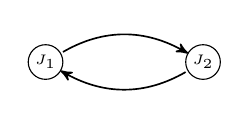
\begin{tikzpicture}[scale = 2]
\tikzstyle{VertexStyle}=[shape = circle,	
							minimum size = 8 pt,
							inner sep = 1.2pt,
                         					draw]
\Vertex[x = 0.0, y = 0.0, L = \tiny {$J_1$}]{v0}
\Vertex[x = 1.0, y = 0.0, L = \tiny {$J_2$}]{v1}
\Edge[style = {bend left, post}](v0)(v1)
\Edge[style = {bend left, post}](v1)(v0)
\end{tikzpicture}


\caption{The reference structure of Jourdain's paradox.}
\end{figure}

As a first pass at defining the reference structure we might simply use the inputs and outputs of the denotation assignment. But we immediately see that this is incorrect. On this approach there would be no sense in which $J_1$ references $J_2$---it would only reference $\neg J_2$. And if $J_1$ referenced $\neg J_2$, then there would be no cyclic reference, since the denotation assignment doesn't map $\neg J_2$ anywhere. Instead we should say that it is in virtue of the denotation assignment mapping $J_1$ to the sentence $\neg J_2$, that $J_1$ references $J_2$. This motivates the following definition.

\begin{defn} We say that a sentence name $\alpha \in \S$ \emph{references} a sentence name $\beta\in \S$ with respect to a denotation assignment $d$ if the name $\beta$ occurs as a syntactic constituent of $d(\alpha)$. 
\end{defn}

With this definition of \textit{referencing}  in play the ``reference structure"  of any given sentence system $(\S,d)$ is best encoded as a directed graph in the following manner.\footnote{A directed graph is just a binary \textit{relation} on a certain domain, i.e. a directed graph $G$ is a pair $(V, E)$ where $E$ is a set of ordered pairs of elements from $V$. For the basics of graph theory see \cite{diestel2010}. We will do our best to not assume that the reader is familiar with graph-theoretic terminology but a quick review of the basics may prove helpful.}

\begin{defn}
Let $\S$ be a set of sentence names and $d$ a denotation assignment.  The \emph{reference graph} $\G_{\S, d}$ is the directed graph with vertex set $\S$ and an edge from $\alpha \in \S$ to $\beta \in \S$ if and only if $\alpha$ references $\beta$.
\end{defn}


For example, we can now represent the reference graph of the Liar paradox as the self-loop, since $d(L) = \neg L$ and $L$ occurs as a syntactic constituent of $\neg L$.


%% self-loop %%

\begin{figure}[ht]
\centering

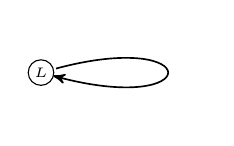
\begin{tikzpicture}[scale = 4]
\tikzstyle{VertexStyle}=[shape = circle,	
								 minimum size = 8pt,
								 inner sep = 1.2pt,
                         draw]

\Vertex[x = 0.0, y = 0.0, L = \tiny {$L$}]{v0}
\Edge[style = {loop right, post}](v0)(v0)
\end{tikzpicture}

\caption{The Liar graph.}
\end{figure}
%%

In Yablo's paradox every sentence $Y_i$ denotes a sentence which has all the sentences names $Y_j$, for $j>i$, as syntactic constituents. So we get the result that in the reference graph every sentence name references every ``later" sentence name.


%% yablo graph %%
\begin{figure}[h]
\centering
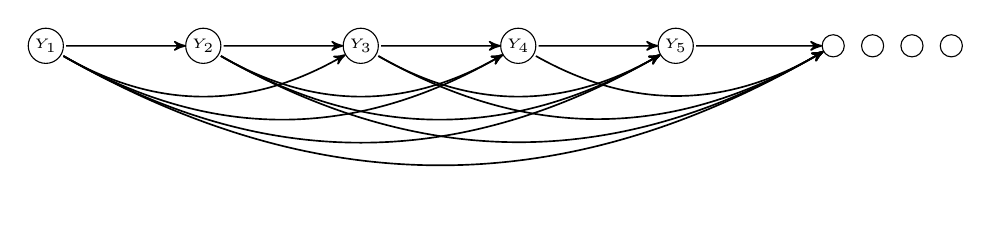
\begin{tikzpicture}[scale = 10]
\tikzstyle{VertexStyle}=[shape = circle,	
								 minimum size = 8 pt,
								 inner sep = 1.2pt,
                         draw]
\Vertex[x = 0.0, y = 0.5, L = \tiny {$Y_1$}]{v0}
\Vertex[x = 0.2, y = 0.5, L = \tiny {$Y_2$}]{v1}
\Vertex[x = 0.4, y = 0.5, L = \tiny {$Y_3$}]{v2}
\Vertex[x = 0.6, y = 0.5, L = \tiny {$Y_4$}]{v3}
\Vertex[x = 0.8, y = 0.5, L = \tiny {$Y_5$}]{v4}
\Vertex[style = {draw = none}, x = 1.0, y = 0.5, L = \tiny {}]{v5}
\Vertex[style = {minimum size = 1 pt}, x = 1.05, y = 0.5, L = \tiny {}]{v6}
\Vertex[style = {minimum size = 1 pt}, x = 1.1, y = 0.5, L = \tiny {}]{v7}
\Vertex[style = {minimum size = 1 pt}, x = 1.15, y = 0.5, L = \tiny {}]{v8}
\Edge[style = {post}](v0)(v1)
\Edge[style = {bend right, post}](v0)(v2)
\Edge[style = {bend right, post}](v0)(v3)
\Edge[style = {bend right, post}](v0)(v4)
\Edge[style = {bend right, post}](v0)(v5)
\Edge[style = {post}](v1)(v2)
\Edge[style = {bend right, post}](v1)(v3)
\Edge[style = {bend right, post}](v1)(v4)
\Edge[style = {bend right, post}](v1)(v5)
\Edge[style = {post}](v2)(v3)
\Edge[style = {bend right, post}](v2)(v4)
\Edge[style = {bend right, post}](v2)(v5)
\Edge[style = {post}](v3)(v4)
\Edge[style = {bend right, post}](v3)(v5)
\Edge[style = {post}](v4)(v5)
\end{tikzpicture}
\caption{The Yablo graph.}
\label{fig:yablo}
\end{figure}
%%

We'd like to provide necessary and sufficient conditions for paradox (hypodox) supporting reference graphs. For a reference graph to ``support" a paradox (hypodox) we mean that there is at least one paradoxical (hypodoxical) sentence system $(\S, d)$ with that reference structure. So the self-loop is paradox and hypodox supporting since the reference graph of both the Liar paradox and the Truth-teller hypodox are isomorphic to the self-loop. This notion of paradox and hypodox supporting graphs is the central concern of this essay. We call paradox supporting graphs \textit{dangerous} and hypodox supporting graphs \textit{precarious}.

\begin{defn} 
We call a directed graph $G$ \emph{dangerous} if there exists a paradoxical sentence system $(\S, d)$ such that $G$ is isomorphic to $\G_{\S, d}$.
\end{defn}

\begin{defn}
We call a directed graph $G$ \emph{precarious} if there exists a hypodoxical sentence system $(\S, d)$ such that $G$ is isomorphic to $\G_{\S, d}$.
\end{defn}

The problem that guides our investigation, then, is this.\\

\textbf{Problem.} \textit{Classify the dangerous (precarious) directed graphs.}


\section{Danger preserving operations}
\label{sec3}

As a first theoretical step toward solving this problem it is useful to find some basic graph operations that preserve danger (precarity). Having these operations at our disposal allows us to separate the wheat from the chaff by reducing complex graphs to simpler---yet still dangerous (precarious)---graphs. In this way we can identify the salient properties and gain a better understanding of the space of dangerous (precarious) graphs. We will make use of these operations throughout the essay to help generate new paradoxes from old ones, find counterexamples to conjectures, and for proving the later theorems.

\subsection{Important graph-theoretic notions}

Here we must introduce some essential graph-theoretic notions. One important concept is that of a vertex's \textit{neighbors}. In a directed graph each vertex has both (i) an associated set of vertices, which are the vertices it points to, (ii) and an associated set of vertices, which are the vertices that point to it. We call these a vertex's \textit{out-neighbors} and \textit{in-neighbors}, respectively.

\begin{defn}
Let $G$ be a directed graph.  We write $N^{+}_G(v)$ for or the set containing exactly the vertices $x$ in $G$ such that there is an edge from $v$ to $x$ ($v$'s out-neighbors) and $N^{-}_G(v)$ for the set containing exactly the vertices $x$ in $G$ such that there is an edge from $x$ to $v$ ($v$'s in-neighbors) .
\end{defn}

%% neighbors %%
\begin{figure}[ht]
\centering
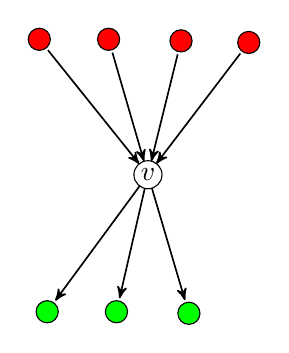
\begin{tikzpicture}[scale = 10]
\tikzstyle{VertexStyle}=[shape = circle,	
								 minimum size = 8pt,
								 inner sep = 1.2pt,
                         draw]
\Vertex[style = {fill = green}, x = 0.351999998092651, y = 0.396000027656555, L = \tiny {}]{v0}
\Vertex[style = {fill = green}, x = 0.439999967813492, y = 0.396000027656555, L = \tiny {}]{v1}
\Vertex[style = {fill = green}, x = 0.531999945640564, y = 0.393999993801117, L = \tiny {}]{v2}
\Vertex[x = 0.479999989271164, y = 0.569999992847443, L = {$v$}]{v3}
\Vertex[style = {fill = red}, x = 0.342000007629395, y = 0.742000013589859, L = \tiny {}]{v4}
\Vertex[style = {fill = red}, x = 0.429999977350235, y = 0.741999983787537, L = \tiny {}]{v5}
\Vertex[style = {fill = red}, x = 0.521999955177307, y = 0.739999979734421, L = \tiny {}]{v6}
\Vertex[style = {fill = red}, x = 0.607999980449677, y = 0.738000005483627, L = \tiny {}]{v7}
\Edge[style = {pre}](v0)(v3)
\Edge[style = {pre}](v1)(v3)
\Edge[style = {pre}](v2)(v3)
\Edge[style = {post}](v4)(v3)
\Edge[style = {post}](v5)(v3)
\Edge[style = {post}](v6)(v3)
\Edge[style = {post}](v7)(v3)
\end{tikzpicture}
\caption{$N^{-}_G(v)$ in red and $N^{+}_G(v)$ in green.}
\end{figure}
%%

Another important notion is that of a \textit{subgraph}. Intuitively, a subgraph of a graph is some ``part" of the graph. But there are different ways to take a part of a graph. You can either take a subset of the vertex set and thrown out some of the edges therein or take a subset of the vertex set and retain all the edges therein. The first is the general notion of a subgraph (i.e. part) and the latter is the more specific concept of an \textit{induced} subgraph (i.e. whole part). More precisely these are defined as follows.

\begin{defn}
Let $G$ be a directed graph.  A \emph{subgraph} $H$ of $G$ is a directed graph with vertex set $V(H)$ a subset of $V(G)$ and edge set $E(H)$ a subset of $E(G)$ such that if $xy \in E(H)$, then $x, y \in H$.  An \emph{induced subgraph} $H$ of $G$ is a subgraph of $G$ such that if $x,y \in H$ and $xy \in E(G)$, then $xy \in E(H)$.  For $A \subseteq V(G)$ we write $G[A]$ for the induced subgraph of $G$ with vertex set $A$.
\end{defn}

\begin{figure}[ht]
\centering
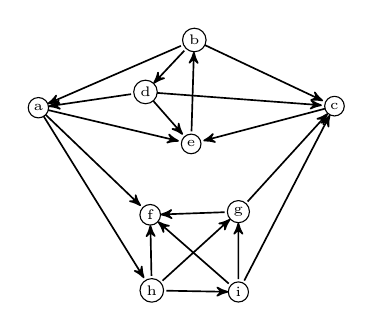
\begin{tikzpicture}[scale = 10]
\tikzstyle{VertexStyle}=[shape = circle,	
								 minimum size = 1pt,
								 inner sep = 1.2pt,
                         draw]
\Vertex[style = {minimum size = 12pt}, x = 0.422000020742416, y = 0.864000007510185, L = \tiny {d}]{v0}
\Vertex[style = {minimum size = 12pt}, x = 0.48400005698204, y = 0.930000007152557, L = \tiny {b}]{v1}
\Vertex[style = {minimum size = 12pt}, x = 0.479999959468842, y = 0.79799996316433, L = \tiny {e}]{v2}
\Vertex[style = {minimum size = 12pt}, x = 0.662000060081482, y = 0.846000000834465, L = \tiny {c}]{v3}
\Vertex[style = {minimum size = 12pt}, x = 0.428000092506409, y = 0.708000034093857, L = \tiny {f}]{v4}
\Vertex[style = {minimum size = 12pt}, x = 0.540000081062317, y = 0.712000042200089, L = \tiny {g}]{v5}
\Vertex[style = {minimum size = 12pt}, x = 0.430000066757202, y = 0.612000018358231, L = \tiny {h}]{v6}
\Vertex[style = {minimum size = 12pt}, x = 0.540000021457672, y = 0.610000044107437, L = \tiny {i}]{v7}
\Vertex[style = {minimum size = 12pt}, x = 0.286000043153763, y = 0.843999996781349, L = \tiny {a}]{v8}
\Edge[style = {post}](v1)(v0)
\Edge[style = {pre}](v2)(v0)
\Edge[style = {pre}](v3)(v0)
\Edge[style = {post}](v2)(v1)
\Edge[style = {pre}](v3)(v1)
\Edge[style = {pre}](v2)(v3)
\Edge[style = {post}](v5)(v4)
\Edge[style = {post}](v6)(v4)
\Edge[style = {post}](v6)(v5)
\Edge[style = {post}](v6)(v7)
\Edge[style = {post}](v7)(v4)
\Edge[style = {post}](v7)(v5)
\Edge[style = {pre}](v4)(v8)
\Edge[style = {pre}](v6)(v8)
\Edge[style = {post}](v5)(v3)
\Edge[style = {post}](v7)(v3)
\Edge[style = {post}](v0)(v8)
\Edge[style = {post}](v1)(v8)
\Edge[style = {pre}](v2)(v8)
\end{tikzpicture}
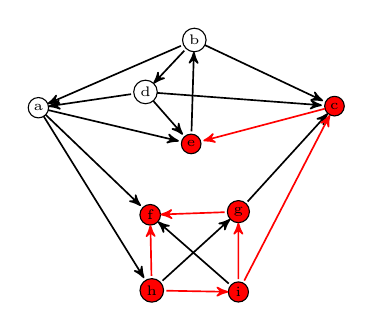
\begin{tikzpicture}[scale = 10]
\tikzstyle{VertexStyle}=[shape = circle,	
								 minimum size = 1pt,
								 inner sep = 1.2pt,
                         draw]
\Vertex[style = {minimum size = 12pt}, x = 0.422000020742416, y = 0.864000007510185, L = \tiny {d}]{v0}
\Vertex[style = {minimum size = 12pt}, x = 0.48400005698204, y = 0.930000007152557, L = \tiny {b}]{v1}
\Vertex[style = {minimum size = 12pt, fill = red}, x = 0.479999959468842, y = 0.79799996316433, L = \tiny {e}]{v2}
\Vertex[style = {minimum size = 12pt, fill = red}, x = 0.662000060081482, y = 0.846000000834465, L = \tiny {c}]{v3}
\Vertex[style = {minimum size = 12pt, fill = red}, x = 0.428000092506409, y = 0.708000034093857, L = \tiny {f}]{v4}
\Vertex[style = {minimum size = 12pt, fill = red}, x = 0.540000081062317, y = 0.712000042200089, L = \tiny {g}]{v5}
\Vertex[style = {minimum size = 12pt, fill = red}, x = 0.430000066757202, y = 0.612000018358231, L = \tiny {h}]{v6}
\Vertex[style = {minimum size = 12pt, fill = red}, x = 0.540000021457672, y = 0.610000044107437, L = \tiny {i}]{v7}
\Vertex[style = {minimum size = 12pt}, x = 0.286000043153763, y = 0.843999996781349, L = \tiny {a}]{v8}
\Edge[style = {post}](v1)(v0)
\Edge[style = {pre}](v2)(v0)
\Edge[style = {pre}](v3)(v0)
\Edge[style = {post}](v2)(v1)
\Edge[style = {pre}](v3)(v1)
\Edge[style = {pre, red}](v2)(v3)
\Edge[style = {post,red}](v5)(v4)
\Edge[style = {post, red}](v6)(v4)
\Edge[style = {post}](v6)(v5)
\Edge[style = {post,red}](v6)(v7)
\Edge[style = {post}](v7)(v4)
\Edge[style = {post, red}](v7)(v5)
\Edge[style = {pre}](v4)(v8)
\Edge[style = {pre}](v6)(v8)
\Edge[style = {post}](v5)(v3)
\Edge[style = {post, red}](v7)(v3)
\Edge[style = {post}](v0)(v8)
\Edge[style = {post}](v1)(v8)
\Edge[style = {pre}](v2)(v8)
\end{tikzpicture}
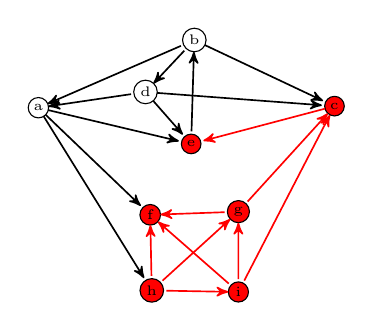
\begin{tikzpicture}[scale = 10]
\tikzstyle{VertexStyle}=[shape = circle,	
								 minimum size = 1pt,
								 inner sep = 1.2pt,
                         draw]
\Vertex[style = {minimum size = 12pt}, x = 0.422000020742416, y = 0.864000007510185, L = \tiny {d}]{v0}
\Vertex[style = {minimum size = 12pt}, x = 0.48400005698204, y = 0.930000007152557, L = \tiny {b}]{v1}
\Vertex[style = {minimum size = 12pt, fill = red}, x = 0.479999959468842, y = 0.79799996316433, L = \tiny {e}]{v2}
\Vertex[style = {minimum size = 12pt, fill = red}, x = 0.662000060081482, y = 0.846000000834465, L = \tiny {c}]{v3}
\Vertex[style = {minimum size = 12pt, fill = red}, x = 0.428000092506409, y = 0.708000034093857, L = \tiny {f}]{v4}
\Vertex[style = {minimum size = 12pt, fill = red}, x = 0.540000081062317, y = 0.712000042200089, L = \tiny {g}]{v5}
\Vertex[style = {minimum size = 12pt, fill = red}, x = 0.430000066757202, y = 0.612000018358231, L = \tiny {h}]{v6}
\Vertex[style = {minimum size = 12pt, fill = red}, x = 0.540000021457672, y = 0.610000044107437, L = \tiny {i}]{v7}
\Vertex[style = {minimum size = 12pt}, x = 0.286000043153763, y = 0.843999996781349, L = \tiny {a}]{v8}
\Edge[style = {post}](v1)(v0)
\Edge[style = {pre}](v2)(v0)
\Edge[style = {pre}](v3)(v0)
\Edge[style = {post}](v2)(v1)
\Edge[style = {pre}](v3)(v1)
\Edge[style = {pre, red}](v2)(v3)
\Edge[style = {post,red}](v5)(v4)
\Edge[style = {post, red}](v6)(v4)
\Edge[style = {post, red}](v6)(v5)
\Edge[style = {post,red}](v6)(v7)
\Edge[style = {post, red}](v7)(v4)
\Edge[style = {post, red}](v7)(v5)
\Edge[style = {pre}](v4)(v8)
\Edge[style = {pre}](v6)(v8)
\Edge[style = {post, red}](v5)(v3)
\Edge[style = {post, red}](v7)(v3)
\Edge[style = {post}](v0)(v8)
\Edge[style = {post}](v1)(v8)
\Edge[style = {pre}](v2)(v8)
\end{tikzpicture}
\caption{A directed graph $G$, a subgraph of $G$ with vertex set $\{c, e, f, g, h, i\}$ and the graph $G[c, e, f, g, h, i]$.}
\end{figure}

Now we turn to the danger preserving operations.

\subsection{Subgraphs}

It seems that a graph should be dangerous (precarious) if and only if some part of it is. We can prove that this is indeed that case. The forward implication is obvious and the reverse implication is proved by assuming that a subgraph of a graph is dangerous (precarious) and then demonstrating a procedure to construct an extended denotation assignment to the whole graph while preserving danger (precarity).

\begin{lem}\label{SubgraphDangerLemma}
Let $G$ be a directed graph.  Then $G$ is dangerous (precarious) if and only if some subgraph of $G$ is dangerous (precarious).
\end{lem}
\begin{proof}
Since $G$ is a subgraph of itself, the forward implication is immediate.  For the reverse implication, let $H$ be a subgraph of $G$ that is dangerous (precarious).  View $V(H)$ as a set of sentence names and let $d$ be a denotation assignment on $V(H)$ such that $(V(H), d)$ is paradoxical (hypodoxical) and
$H = \G_{V(H), d}$.

We construct a denotation assignment $d'$ on $V(G)$ by employing ``junk conjunctions" $J_x = \bot \wedge \bigwedge_{y \in N^{+}_G(x)} y$, for each $x \in V(G)$. The denotation assignment $d'$ assigns to $x$ a sentence containing its junk conjunction---it is clear that this gets the referencing right, but the junk sentences must be added in such a way that they have no impact on the acceptability of truth-value assignments. For $x \in V(G)$, let

\[d'(x) = \begin{cases}
d(x) \vee J_x & \text{if } x \in V(H) \\
J_x & \text{if } x \not \in V(H)
\end{cases}.\]

Then, by construction, $G = \G_{V(G), d'}$ and $(V(G), d')$ is paradoxical (hypodoxical).  Hence $G$ is dangerous (precarious).
\end{proof}

For an example, consider the following version of Curry's paradox.  Put $\S = \{A, B\}$, $d(A) = \neg A \vee B$ and $d(B) = \bot$.  The reference graph of $(\S, d)$ is given in Figure \ref{fig:curry}.  By Lemma \ref{SubgraphDangerLemma}, we can determine that this graph is dangerous prior to considering Curry's paradox, since it has the self-loop as a subgraph.
\begin{figure}[ht]
\centering

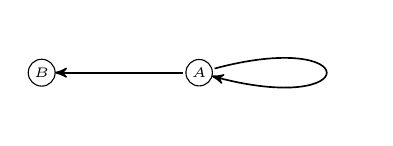
\begin{tikzpicture}[scale = 4]
\tikzstyle{VertexStyle}=[shape = circle,	
								 minimum size = 8pt,
								 inner sep = 1.2pt,
                         draw]

\Vertex[x = 0.5, y = 0.0, L = \tiny {$A$}]{v0}
\Vertex[x = 0.0, y = 0.0, L = \tiny {$B$}]{v1}
\Edge[style = {loop right, post}](v0)(v0)
\Edge[style = {post}](v0)(v1)
\end{tikzpicture}
\caption{The Curry graph.}
\label{fig:curry}
\end{figure}

Above we added junk conjunctions, which did the trick because they established the right reference relation while not affecting the acceptability of truth-assignments on the sentence system. They were able to do this because on every truth-assignment they got the same value, i.e. they were \textit{constant}.  We would also like to be able to remove constant junk from a sentence system, thereby eliminating certain reference relations without affecting the acceptability of truth-assignments. 

\prg For example, for the system $\S = {A}$ and $d(A) = A \wedge \neg A$ we can modify $d$ to $d'(A) = \bot$ thereby removing the reference relations without affecting the acceptability of truth-value assignments. If this procedure is carried out for all the constant junk in a sentence system, we will say that the system is \textit{junk-free}.\footnote{Note that a system that is junk-free may still include ``junky disjuncts" such as in the right disjunct of $B \vee (A \wedge\neg A)$. Junk-free sentence systems are merely free of \textit{constant} junk.}  Let's define this notion and prove a lemma, while we are on the topic of ``junk".

\begin{defn}
A sentence system $(\S, d)$ is \emph{junk-free} if and only if for every $\alpha \in \S$, if $d(\alpha) \not \in \{\bot, \top\}$, then there exist truth assignments $v_0, v_1$ on $\S$ such that $\llbracket d(\alpha)\rrbracket(v_0) = 0$ and  $\llbracket d(\alpha)\rrbracket(v_1) = 1$.
\end{defn}

Since removing junk does not affect the acceptability of truth-assignments on a system, the removal of junk preserves the paradoxicality (hypodoxicality) of a sentence system.

\begin{lem}\label{JunkRemoval}
Let the system $(\S, d)$ be paradoxical (hypodoxical).  Then there is a denotation assignment $d'$ on $\S$ such that $(\S, d')$ is junk-free, paradoxical (hypodoxical) and $\G_{\S, d'}$ is a subgraph of $\G_{\S, d}$.
\end{lem}
\begin{proof}
Assume $(\S, d)$ is paradoxical (hypodoxical). Let $J$ be the set of $\alpha \in \S$ such that there is $t_{\alpha} \in \{0, 1\}$ so that $\llbracket d(\alpha) \rrbracket(v) = t_{\alpha}$ for each $v \in \V_\S$.  For each $\alpha \not \in J$, let $d'(\alpha) = d(\alpha)$ and for $\alpha \in J$, let 

\[d'(\alpha) = \begin{cases}
\bot & \text{if } t_{\alpha} = 0 \\
\top & \text{if }  t_{\alpha} = 1
\end{cases}.\]

Then, by construction, $(\S, d')$ is junk-free, paradoxical (hypodoxical) and $\G_{\S, d'}$ is a subgraph of $\G_{\S, d}$.
\end{proof}

\subsection{Smoothing and subdividing}

For a sentence system $(\S, d)$, intuitively, we can ``simplify'' it to the system $(\S', d')$ by picking some $\alpha \in \S$, replacing every occurance of $\alpha$ with $d(\alpha)$ and then removing $\alpha$ from $\S$.  Doing so gives rise to an additional danger preserving operation on graphs.  This is supported by the following lemma.

\begin{lem}\label{SubstitutionLemma}
Let $\S$ be a set and let $\psi \in \S^+$.  Let $v$ be a truth-value assignment on $\S$.  Let $\left\{ (\alpha_i, \gamma_i)\right\}_{i \in I} \subseteq \S \times \S^+$ such that the $\alpha_i$ are pairwise distinct. If $v(\alpha_i) = \llbracket \gamma_i \rrbracket(v)$ for each $i \in I$, then

\[\left\llbracket \psi\left[\alpha_i \Rightarrow \gamma_i \mid i \in I\right]\right\rrbracket(v) = \llbracket \psi \rrbracket(v).\] 
\end{lem}
\begin{proof}
This is immediate from the definition of the semantics.
\end{proof}

Now consider a pair $(\S, d)$ and $\alpha \in \S$ such that $\alpha$ does not occur as a constituent of $d(\alpha)$. Let $\S' = \S - \{\alpha\}$ and for $\beta \in \S'$ let $d'(\beta) = d(\beta)\left[\alpha \Rightarrow d(\alpha)\right]$.  Then $d'$ is a denotation assignment on $\S'$. Given a truth assignment $v$ on $\S$, let $v'$ be $v$ restricted to $S'$.  Then, by Lemma \ref{SubstitutionLemma}, $v$ is acceptable on $\S$ relative to $d$ if and only if $v'$ is acceptable on $\S'$ relative to $d'$.  Thus the following ``smoothing'' operation leaves dangerous graphs dangerous and precarious graphs precarious.

\begin{defn}
Let $G$ be a directed graph.  Let $y \in V(G)$ such that $yy \not \in E(G)$.  The \emph{smoothing} of $G$ at $y$ is the graph $H$ with $V(H) = V(G) - y$ and
$E(H) = E(G - y) \cup \left\{ab \mid a \in N^-(y), b \in N^+(y)\right\}$.
\end{defn}

%% smoothing %%
\tikzstyle{VertexStyle}=[shape = circle,	
  								 minimum size = 1pt,
								 inner sep = 1.2pt,
								 draw]

\begin{figure}[ht]
\centering
\subfloat[] {
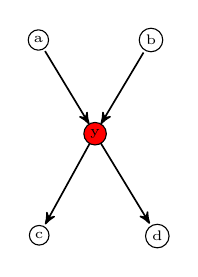
\begin{tikzpicture}[scale = 10]
\tikzstyle{VertexStyle}=[shape = circle,	
								 minimum size = 1pt,
								 inner sep = 1.2pt,
                         draw]
\Vertex[x = 0.219333365559578, y = 0.701000034809113, L = \tiny {c}]{v0}
\Vertex[x = 0.369333326816559, y = 0.699999988079071, L = \tiny {d}]{v1}
\Vertex[style = {fill=red}, x = 0.290333330631256, y = 0.830000028014183, L = \tiny {y}]{v2}
\Vertex[x = 0.218333393335342, y = 0.949000023305416, L = \tiny {a}]{v3}
\Vertex[x = 0.361333340406418, y = 0.948999986052513, L = \tiny {b}]{v4}
\Edge[style = {post}](v3)(v2)
\Edge[style = {post}](v4)(v2)
\Edge[style = {pre}](v0)(v2)
\Edge[style = {pre}](v1)(v2)
\end{tikzpicture}
}
\subfloat[] {
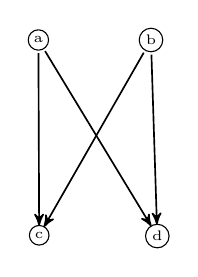
\begin{tikzpicture}[scale = 10]
\tikzstyle{VertexStyle}=[shape = circle,	
								 minimum size = 1pt,
								 inner sep = 1.2pt,
                         draw]
\Vertex[x = 0.219333365559578, y = 0.701000034809113, L = \tiny {c}]{v0}
\Vertex[x = 0.369333326816559, y = 0.699999988079071, L = \tiny {d}]{v1}
\Vertex[x = 0.218333393335342, y = 0.949000023305416, L = \tiny {a}]{v2}
\Vertex[x = 0.361333340406418, y = 0.948999986052513, L = \tiny {b}]{v3}
\Edge[style = {post}](v2)(v0)
\Edge[style = {post}](v3)(v0)
\Edge[style = {post}](v2)(v1)
\Edge[style = {post}](v3)(v1)
\end{tikzpicture}
}
\caption{A graph and its smoothing at $y$.}
\end{figure}
%%

The reverse operation of introducing a new name doesn't behave nicely in general, but it does in a few interesting special cases. One is that of a subdivision.

\begin{defn}
Let $G$ be a directed graph.  A \emph{subdivision} of $G$ is a graph formed by replacing each edge $xy$ of $G$ with a path $p_{xy}$ from $x$ to $y$.  Note that we allow $p_{xy}$ to be length $1$; that is, $p_{xy} = xy$.
\end{defn}

% subdivision %

\begin{figure}[ht]
\centering
\subfloat[] {
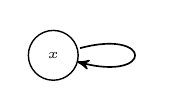
\begin{tikzpicture}[scale = 2]

\Vertex[x = 0.0, y = 0.0, L = \tiny {$x$}]{v0}
\Edge[style = {loop right, post}](v0)(v0)
\end{tikzpicture}
}
\subfloat[] {
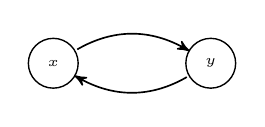
\begin{tikzpicture}[scale = 2]
\Vertex[x = 0.0, y = 0.0, L = \tiny {$x$}]{v0}
\Vertex[style = {fill = green}, x = 1.0, y = 0.0, L = \tiny {$y$}]{v1}
\Edge[style = {bend left, post}](v0)(v1)
\Edge[style = {bend left, post}](v1)(v0)
\end{tikzpicture}
}
\subfloat[] {
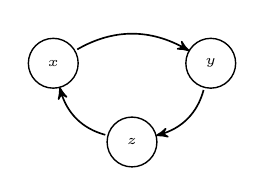
\begin{tikzpicture}[scale = 2]
\Vertex[x = 0.0, y = 0.0, L = \tiny {$x$}]{v0}
\Vertex[x = 1.0, y = 0.0, L = \tiny {$y$}]{v1}
\Vertex[style = {fill = green}, x = 0.5, y = -0.5, L = \tiny {$z$}]{v2}
\Edge[style = {bend left, post}](v0)(v1)
\Edge[style = {bend left, post}](v1)(v2)
\Edge[style = {bend left, post}](v2)(v0)
\end{tikzpicture}
}
\caption{The Liar graph and two subdivisions.}
\end{figure}
%%

\begin{lem}\label{SubdivisionLemma}
A subdivision of a directed graph $G$ is dangerous if and only if $G$ is.\footnote{This also holds for precarious graphs but we omit the proof here as it turns out to be quite nasty to write down---and in any case follows trivially from the later results about precarity and groundedness (see Theorem \ref{PrecariousCharacterization}). Similar remarks apply to precarity's status as a topological property.}
\end{lem}
\begin{proof}
First, assume $G$ is dangerous and let $d$ be a denotation assignment on $V(G)$ such that $G = \G_{V(G), d}$ and $(V(G), d)$ is paradoxical.  Let $H$ be the subdivision of $G$ where each edge $xy \in E(G)$ is replaced with the path $p_{xy}$ from $x$ to $y$.  Say the vertices of $p_{xy}$ in order are $x = z_{xy}^1, z_{xy}^2, \ldots, z_{xy}^{k_{xy}} = y$.  Define a denotation assignment $d'$ on $V(H)$ by

\[d'(w) = \begin{cases}
d(w)[y \Rightarrow z_{wy}^2 \mid wy \in E(G)] & \text{if } w \in V(G) \\
z_{xy}^{j+1} & \text{if } w = z_{xy}^j \text{ for } xy \in E(G), j \geq 2. \\
\end{cases}\]

By construction we have $H = \G_{V(H), d'}$.  Now we will show that $H$ is paradoxical with this denotation assignment.  Assume not and let $v'$ be an acceptable truth assignment on $V(H)$ with respect to $d'$ and let $v$ be $v'$ restricted to $V(G)$. Then for each $xy \in E(G)$ and $2 \leq j < k_{xy}$ we have $\llbracket d'(z_{xy}^j) \rrbracket(v') = \llbracket z_{xy}^{j + 1} \rrbracket(v')$.  Hence $v'(z_{xy}^2) = \llbracket d'(z_{xy}^2) \rrbracket(v') = \llbracket d'(y) \rrbracket(v') = v'(y)$ since $v'$ is acceptable.  Thus for $w \in V(G)$, by Lemma \ref{SubstitutionLemma}, we have $v(w) = v'(w) = \llbracket d'(w) \rrbracket(v') = \llbracket d(w)[y \Rightarrow z_{wy}^2 \mid wy \in E(G)] \rrbracket(v') = \llbracket d(w) \rrbracket(v') = \llbracket d(w) \rrbracket(v)$.  Whence $v$ is acceptable on $V(G)$ with respect to $d$.  This contradicts the fact that $G$ is dangerous.

The other direction is very similar, basically we smooth at all of the subdivision vertices.  We omit the proof to avoid unnecessary tedium.
\end{proof}

We should mention here that the fact that subdivision preserves danger entails that danger is preserved under homeomorphisms and thus that being dangerous is a \textit{topological property} of directed graphs.  The terms ``homeomorphism'' and ``topological property'' are usually applied topological spaces and in particular undirected graphs.  Even though a directed graph is not a topological space, the straightforward generalization of the definitions gives a useful concept.

\begin{defn}
Two directed graphs $G$ and $H$ are \emph{homeomorphic} if some subdivision of $G$ is isomorphic to some subdivision of $H$.
\end{defn}

\begin{lem}
If $G$ and $H$ are homeomorphic directed graphs, then $G$ is dangerous if and only if $H$ is dangerous.
\end{lem}
\begin{proof}
Assume $G$ and $H$ are homeomorphic directed graphs and let $G'$ and $H'$ be subdivisions of $G$ and $H$ respectively such that $G'$ is isomorphic to $H'$. The lemma follows by applying Lemma \ref{SubdivisionLemma} to $G$ and $G'$ and to $H$ and $H'$.
\end{proof}

\subsection{Unwinding}
We give a construction that turns any finite paradoxical sentence system into an infinite acyclic paradoxical sentence system.\footnote{Note that Cook's \cite{cook} proof of his unwinding theorem regarding $F$-systems works for unwindings of infinitary systems as well as finitary ones. The cases where unwinding would fail in the infinite case are related to Schlenker's \cite{schlenker2007elimination} discussion of the elimination of self-reference.}  Following \cite{cook}\footnote{\cite{cook} attributes the basic idea of ``unwinding" to Thomas Bolander who we know (from personal communication) also has some unpublished results on the graph-theoretic nature of paradox supporting structures. We in turn owe the idea of unwinding to Bolander via \cite{cook}.}, we call this construction \textit{unwinding the paradox} (see Figure \ref{fig:unwinding}). Cook gives a nice description of the philosophical import of unwinding.

\begin{quote}
The notion of unwinding sheds considerable light onto the relevance of Yablo's paradox to debates regarding the connections between paradox and circularity. Prior to Yablo's discovery, semantic paradox was thought by most to be inextricably linked to circularity.  Post Yablo, however, it is fair to say that most philosophers of language and logic think of the infinite non-circular construction as an isolated curiosity. Unwinding finite paradoxes, however, demonstrates that infinite non-circular constructions can be associated with each instance of a wide class of circular finite paradoxes. As a result, we might be forced to reconsider the assumption that circularity has any fundamental connection to the logical and philosophical problems associated with truth.\footnote{\cite{cook}, p. 772.}
\end{quote}

In what follows we show that an infinite non-circular construction can be associated with each finite paradox. More precisely, we show that from any finite paradoxocial (hypodoxical) sentence system we can get an infinite \textit{acyclic} paradoxocial (hypodoxical) sentence system that is paradoxical (hypodoxical) for essentially the same reason.

\begin{defn}
Let $G$ be a finite directed graph and let $<$ be a total order on $V(G)$.  Define an ordering on $V(G) \times \mathbb{N}$ by $(x_1, i) < (x_2, j)$ if and only if $i < j$ or $i = j$ and $x_1 < x_2$. The \emph{unwinding} of $G$ is the graph with vertex set $V(G) \times \mathbb{N}$ with an edge from $(x_1, i)$ to $(x_2, j)$ if and only if $x_1x_2 \in E(G)$ and $(x_1, i) < (x_2, j)$.  We denote the unwinding of $G$ with respect to the ordering $<$ by $u_{<}(G)$.
\end{defn}

\begin{figure}[ht]
\centering
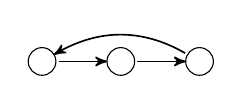
\begin{tikzpicture}[scale = 10]
\tikzstyle{VertexStyle}=[
shape = circle, 
minimum size = 10pt,
inner sep = 1.2pt,
draw]
\Vertex[x = 0, y = 0, L = \tiny {}]{v0}
\Vertex[x = 0.1, y = 0, L = \tiny {}]{v1}
\Vertex[x = 0.2, y = 0, L = \tiny {}]{v2}
\Edge[style = {post}](v0)(v1)
\Edge[style = {post}](v1)(v2)
\Edge[style = {post, bend right}](v2)(v0)
\end{tikzpicture}
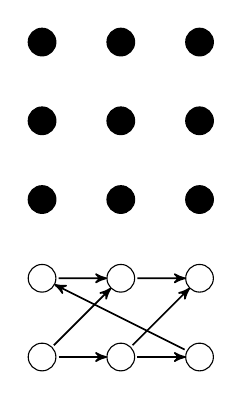
\begin{tikzpicture}[scale = 10]
\tikzstyle{VertexStyle}=[
shape = circle, 
minimum size = 10pt,
inner sep = 1.2pt,
draw]
\Vertex[x = 0, y = 0, L = \tiny {}]{v3}
\Vertex[x = 0.1, y = 0, L = \tiny {}]{v4}
\Vertex[x = 0.2, y = 0, L = \tiny {}]{v5}
\Vertex[x = 0, y = 0.1, L = \tiny {}]{v6}
\Vertex[x = 0.1, y = 0.1, L = \tiny {}]{v7}
\Vertex[x = 0.2, y = 0.1, L = \tiny {}]{v8}
\Vertex[style = {fill = black, minimum size = 1pt}, x = 0, y = 0.2, L = \tiny {}]{v12}
\Vertex[style = {fill = black, minimum size = 1pt}, x = 0.1, y = 0.2, L = \tiny {}]{v13}
\Vertex[style = {fill = black, minimum size = 1pt}, x = 0.2, y = 0.2, L = \tiny {}]{v14}
\Vertex[style = {fill = black, minimum size = 1pt}, x = 0, y = 0.3, L = \tiny {}]{v18}
\Vertex[style = {fill = black, minimum size = 1pt}, x = 0.1, y = 0.3, L = \tiny {}]{v19}
\Vertex[style = {fill = black, minimum size = 1pt}, x = 0.2, y = 0.3, L = \tiny {}]{v20}
\Vertex[style = {fill = black, minimum size = 1pt}, x = 0, y = 0.4, L = \tiny {}]{v24}
\Vertex[style = {fill = black, minimum size = 1pt}, x = 0.1, y = 0.4, L = \tiny {}]{v25}
\Vertex[style = {fill = black, minimum size = 1pt}, x = 0.2, y = 0.4, L = \tiny {}]{v26}
\Edge[style = {post}](v3)(v4)
\Edge[style = {post}](v4)(v5)
\Edge[style = {post}](v6)(v7)
\Edge[style = {post}](v7)(v8)
\Edge[style = {post}](v3)(v7)
\Edge[style = {post}](v4)(v8)
\Edge[style = {post}](v5)(v6)
\end{tikzpicture}
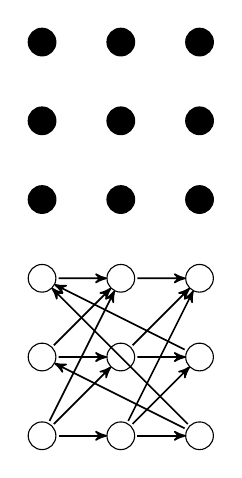
\begin{tikzpicture}[scale = 10]
\tikzstyle{VertexStyle}=[
shape = circle, 
minimum size = 10pt,
inner sep = 1.2pt,
draw]
\Vertex[x = 0, y = 0, L = \tiny {}]{v3}
\Vertex[x = 0.1, y = 0, L = \tiny {}]{v4}
\Vertex[x = 0.2, y = 0, L = \tiny {}]{v5}
\Vertex[x = 0, y = 0.1, L = \tiny {}]{v6}
\Vertex[x = 0.1, y = 0.1, L = \tiny {}]{v7}
\Vertex[x = 0.2, y = 0.1, L = \tiny {}]{v8}
\Vertex[x = 0, y = 0.2, L = \tiny {}]{v9}
\Vertex[x = 0.1, y = 0.2, L = \tiny {}]{v10}
\Vertex[x = 0.2, y = 0.2, L = \tiny {}]{v11}
\Vertex[style = {fill = black, minimum size = 1pt}, x = 0, y = 0.3, L = \tiny {}]{v15}
\Vertex[style = {fill = black, minimum size = 1pt}, x = 0.1, y = 0.3, L = \tiny {}]{v16}
\Vertex[style = {fill = black, minimum size = 1pt}, x = 0.2, y = 0.3, L = \tiny {}]{v17}
\Vertex[style = {fill = black, minimum size = 1pt}, x = 0, y = 0.4, L = \tiny {}]{v21}
\Vertex[style = {fill = black, minimum size = 1pt}, x = 0.1, y = 0.4, L = \tiny {}]{v22}
\Vertex[style = {fill = black, minimum size = 1pt}, x = 0.2, y = 0.4, L = \tiny {}]{v23}
\Vertex[style = {fill = black, minimum size = 1pt}, x = 0, y = 0.5, L = \tiny {}]{v27}
\Vertex[style = {fill = black, minimum size = 1pt}, x = 0.1, y = 0.5, L = \tiny {}]{v28}
\Vertex[style = {fill = black, minimum size = 1pt}, x = 0.2, y = 0.5, L = \tiny {}]{v29}
\Edge[style = {post}](v3)(v4)
\Edge[style = {post}](v4)(v5)
\Edge[style = {post}](v6)(v7)
\Edge[style = {post}](v7)(v8)
\Edge[style = {post}](v3)(v7)
\Edge[style = {post}](v4)(v8)
\Edge[style = {post}](v5)(v6)
\Edge[style = {post}](v9)(v10)
\Edge[style = {post}](v10)(v11)
\Edge[style = {post}](v3)(v10)
\Edge[style = {post}](v4)(v11)
\Edge[style = {post}](v5)(v9)
\Edge[style = {post}](v6)(v10)
\Edge[style = {post}](v7)(v11)
\Edge[style = {post}](v8)(v9)
\end{tikzpicture}
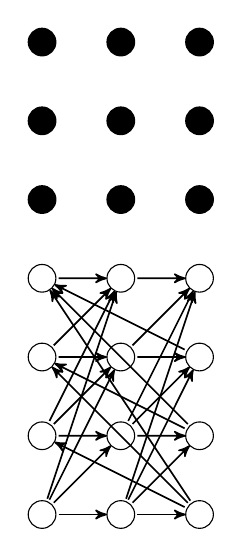
\begin{tikzpicture}[scale = 10]
\tikzstyle{VertexStyle}=[
shape = circle, 
minimum size = 10pt,
inner sep = 1.2pt,
draw]
\Vertex[x = 0, y = 0, L = \tiny {}]{v3}
\Vertex[x = 0.1, y = 0, L = \tiny {}]{v4}
\Vertex[x = 0.2, y = 0, L = \tiny {}]{v5}
\Vertex[x = 0, y = 0.1, L = \tiny {}]{v6}
\Vertex[x = 0.1, y = 0.1, L = \tiny {}]{v7}
\Vertex[x = 0.2, y = 0.1, L = \tiny {}]{v8}
\Vertex[x = 0, y = 0.2, L = \tiny {}]{v9}
\Vertex[x = 0.1, y = 0.2, L = \tiny {}]{v10}
\Vertex[x = 0.2, y = 0.2, L = \tiny {}]{v11}
\Vertex[x = 0, y = 0.3, L = \tiny {}]{v12}
\Vertex[x = 0.1, y = 0.3, L = \tiny {}]{v13}
\Vertex[x = 0.2, y = 0.3, L = \tiny {}]{v14}
\Vertex[style = {fill = black, minimum size = 1pt}, x = 0, y = 0.4, L = \tiny {}]{v18}
\Vertex[style = {fill = black, minimum size = 1pt}, x = 0.1, y = 0.4, L = \tiny {}]{v19}
\Vertex[style = {fill = black, minimum size = 1pt}, x = 0.2, y = 0.4, L = \tiny {}]{v20}
\Vertex[style = {fill = black, minimum size = 1pt}, x = 0, y = 0.5, L = \tiny {}]{v24}
\Vertex[style = {fill = black, minimum size = 1pt}, x = 0.1, y = 0.5, L = \tiny {}]{v25}
\Vertex[style = {fill = black, minimum size = 1pt}, x = 0.2, y = 0.5, L = \tiny {}]{v26}
\Vertex[style = {fill = black, minimum size = 1pt}, x = 0, y = 0.6, L = \tiny {}]{v30}
\Vertex[style = {fill = black, minimum size = 1pt}, x = 0.1, y = 0.6, L = \tiny {}]{v31}
\Vertex[style = {fill = black, minimum size = 1pt}, x = 0.2, y = 0.6, L = \tiny {}]{v32}
\Edge[style = {post}](v3)(v4)
\Edge[style = {post}](v4)(v5)
\Edge[style = {post}](v6)(v7)
\Edge[style = {post}](v7)(v8)
\Edge[style = {post}](v3)(v7)
\Edge[style = {post}](v4)(v8)
\Edge[style = {post}](v5)(v6)
\Edge[style = {post}](v9)(v10)
\Edge[style = {post}](v10)(v11)
\Edge[style = {post}](v3)(v10)
\Edge[style = {post}](v4)(v11)
\Edge[style = {post}](v5)(v9)
\Edge[style = {post}](v6)(v10)
\Edge[style = {post}](v7)(v11)
\Edge[style = {post}](v8)(v9)
\Edge[style = {post}](v12)(v13)
\Edge[style = {post}](v13)(v14)
\Edge[style = {post}](v3)(v13)
\Edge[style = {post}](v4)(v14)
\Edge[style = {post}](v5)(v12)
\Edge[style = {post}](v6)(v13)
\Edge[style = {post}](v7)(v14)
\Edge[style = {post}](v8)(v12)
\Edge[style = {post}](v9)(v13)
\Edge[style = {post}](v10)(v14)
\Edge[style = {post}](v11)(v12)
\end{tikzpicture}
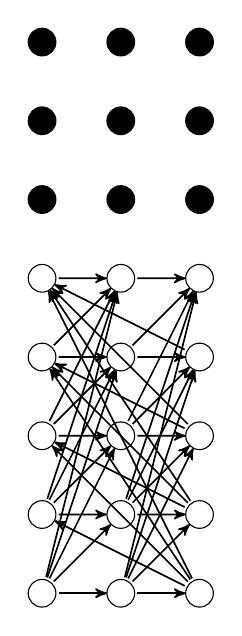
\begin{tikzpicture}[scale = 10]
\tikzstyle{VertexStyle}=[
shape = circle, 
minimum size = 10pt,
inner sep = 1.2pt,
draw]
\Vertex[x = 0, y = 0, L = \tiny {}]{v3}
\Vertex[x = 0.1, y = 0, L = \tiny {}]{v4}
\Vertex[x = 0.2, y = 0, L = \tiny {}]{v5}
\Vertex[x = 0, y = 0.1, L = \tiny {}]{v6}
\Vertex[x = 0.1, y = 0.1, L = \tiny {}]{v7}
\Vertex[x = 0.2, y = 0.1, L = \tiny {}]{v8}
\Vertex[x = 0, y = 0.2, L = \tiny {}]{v9}
\Vertex[x = 0.1, y = 0.2, L = \tiny {}]{v10}
\Vertex[x = 0.2, y = 0.2, L = \tiny {}]{v11}
\Vertex[x = 0, y = 0.3, L = \tiny {}]{v12}
\Vertex[x = 0.1, y = 0.3, L = \tiny {}]{v13}
\Vertex[x = 0.2, y = 0.3, L = \tiny {}]{v14}
\Vertex[x = 0, y = 0.4, L = \tiny {}]{v15}
\Vertex[x = 0.1, y = 0.4, L = \tiny {}]{v16}
\Vertex[x = 0.2, y = 0.4, L = \tiny {}]{v17}
\Vertex[style = {fill = black, minimum size = 1pt}, x = 0, y = 0.5, L = \tiny {}]{v21}
\Vertex[style = {fill = black, minimum size = 1pt}, x = 0.1, y = 0.5, L = \tiny {}]{v22}
\Vertex[style = {fill = black, minimum size = 1pt}, x = 0.2, y = 0.5, L = \tiny {}]{v23}
\Vertex[style = {fill = black, minimum size = 1pt}, x = 0, y = 0.6, L = \tiny {}]{v27}
\Vertex[style = {fill = black, minimum size = 1pt}, x = 0.1, y = 0.6, L = \tiny {}]{v28}
\Vertex[style = {fill = black, minimum size = 1pt}, x = 0.2, y = 0.6, L = \tiny {}]{v29}
\Vertex[style = {fill = black, minimum size = 1pt}, x = 0, y = 0.7, L = \tiny {}]{v33}
\Vertex[style = {fill = black, minimum size = 1pt}, x = 0.1, y = 0.7, L = \tiny {}]{v34}
\Vertex[style = {fill = black, minimum size = 1pt}, x = 0.2, y = 0.7, L = \tiny {}]{v35}
\Edge[style = {post}](v3)(v4)
\Edge[style = {post}](v4)(v5)
\Edge[style = {post}](v6)(v7)
\Edge[style = {post}](v7)(v8)
\Edge[style = {post}](v3)(v7)
\Edge[style = {post}](v4)(v8)
\Edge[style = {post}](v5)(v6)
\Edge[style = {post}](v9)(v10)
\Edge[style = {post}](v10)(v11)
\Edge[style = {post}](v3)(v10)
\Edge[style = {post}](v4)(v11)
\Edge[style = {post}](v5)(v9)
\Edge[style = {post}](v6)(v10)
\Edge[style = {post}](v7)(v11)
\Edge[style = {post}](v8)(v9)
\Edge[style = {post}](v12)(v13)
\Edge[style = {post}](v13)(v14)
\Edge[style = {post}](v3)(v13)
\Edge[style = {post}](v4)(v14)
\Edge[style = {post}](v5)(v12)
\Edge[style = {post}](v6)(v13)
\Edge[style = {post}](v7)(v14)
\Edge[style = {post}](v8)(v12)
\Edge[style = {post}](v9)(v13)
\Edge[style = {post}](v10)(v14)
\Edge[style = {post}](v11)(v12)
\Edge[style = {post}](v15)(v16)
\Edge[style = {post}](v16)(v17)
\Edge[style = {post}](v3)(v16)
\Edge[style = {post}](v4)(v17)
\Edge[style = {post}](v5)(v15)
\Edge[style = {post}](v6)(v16)
\Edge[style = {post}](v7)(v17)
\Edge[style = {post}](v8)(v15)
\Edge[style = {post}](v9)(v16)
\Edge[style = {post}](v10)(v17)
\Edge[style = {post}](v11)(v15)
\Edge[style = {post}](v12)(v16)
\Edge[style = {post}](v13)(v17)
\Edge[style = {post}](v14)(v15)
\end{tikzpicture}
\caption{The $3$-cycle and its unwinding at various stages.}
\label{fig:unwinding}
\end{figure}

\begin{lem}\label{UnrollingKillsCycles}
Let $G$ be a finite directed graph and let $<$ be a total order on $V(G)$.  Then
$u_{<}(G)$ is acyclic.
\end{lem}
\begin{proof}
Assume there is a directed cycle in $u_{<}(G)$ with vertices $(x_1, i_1), (x_2, y_1), \ldots, (x_k, i_k), (x_1, i_1)$.  Then by the definition of the edge set of $u_{<}(G)$, we have $(x_1, i_1) < (x_2, y_1) < \cdots < (x_k, i_k) < (x_1, i_1)$, a contradiction.  Hence there is no directed cycle.
\end{proof}

\begin{lem}\label{UnrollingPreservesDanger}
Let $G$ be a finite directed graph and let $<$ be a total order on $V(G)$.  Then $G$ is dangerous (precarious) if and only if $u_{<}(G)$ is dangerous (precarious).
\end{lem}
\begin{proof}
Let $d$ be a denotation assignment on $V(G)$.  Define a denotation assignment $d'$ on $V(G) \times \mathbb{N}$ as follows. For $x \in V(G)$ and $k \in \mathbb{N}$, put 
\[T_{x, k} = d(x)\left[t \Rightarrow (t, k + 1) \mid t \leq x\right]\left[t \Rightarrow (t, k) \mid t > x\right].\]

That is, in the sentence $d(x)$, we replace each $t \in V(G)$ which is at most $x$ with $(t, k + 1) \in V(G) \times \mathbb{N}$ and then replace each each $t \in V(G)$ which is greater than $x$ with $(t, k) \in V(G) \times \mathbb{N}$. This gets the referencing to match the unwinding graph.

Now for $(x, k) \in V(G) \times \mathbb{N}$, let $d'((x,k)) = \bigwedge_{j \geq k} T_{x, j}$. Then, by construction, $\G_{V(G) \times \mathbb{N}, d'} = u_{<}(G)$.

We first show that if $G$ is not dangerous (precarious) then $u_{<}(G)$ is not dangerous (precarious). Assume $G$ is not dangerous (precarious). Let $v$ be an acceptable truth assignment on $V(G)$ with respect to $d$.  Define a truth assignment $v'$ on $V(G) \times \mathbb{N}$ by setting $v'((x, k)) = v(x)$.  Then
\begin{align*}
\llbracket d'((x,k)) \rrbracket (v') &= \bigwedge_{j \geq k}  \llbracket T_{x, j} \rrbracket (v') \\
&=  \bigwedge_{j \geq k} d(x)\left[t \Rightarrow v'((t, k + 1)) \mid t \leq x \right]\left[t \Rightarrow v'((t, k))\mid t > x\right] \\
&=  \bigwedge_{j \geq k} d(x)\left[t \Rightarrow v(t) \mid t \leq x \right]\left[t \Rightarrow v(t)\mid t > x\right] \\
&= \bigwedge_{j \geq k} \llbracket d(x) \rrbracket(v) \\
&=  \llbracket d(x) \rrbracket(v) \\
&= v(x) \\
& = v'((x, k))
\end{align*}
Hence $v'$ is acceptable with respect to $d'$.   Hence $u_{<}(G)$ is not dangerous. To see that $u_{<}(G)$ is not precarious, note that if $v_1$ and $v_2$ are distinct acceptable truth assignments on $V(G)$, then $v_1'$ and $v_2'$ are distinct as well.

Now for the other direction, assume that $u_{<}(G)$ is not dangerous (precarious). Let $v'$ be an acceptable truth assignment on $V(G) \times \mathbb{N}$ with respect to $d'$.

We claim that for each $x \in V(G)$, we have $v'((x, k_1)) = v'((x, k_2))$ for all $k_1, k_2 \in \mathbb{N}$.  Let $x \in V(G)$.  Assume $v'((x, k)) = 1$ for some $k \in \mathbb{N}$ and let $j \geq k$. We have $1 = v'((x,k)) = \llbracket d'((x,k))\rrbracket(v') = \llbracket d'(x, j) \wedge \bigwedge_{k \leq i < j} T_{x, i}\rrbracket(v')$.  Hence $v'(x, j) = \llbracket d'(x, j)\rrbracket(v') = 1$. Hence for each $x \in V(G)$ we have $M_x \in \mathbb{N}$ such that either $v'((x , j)) = 1$ for all $j \geq M_x$ or $v'((x, j)) = 0$ for all $j \in \mathbb{N}$.  Since $G$ is finite, we can define $M = \max_{x \in V(G)} M_x$.  To get a contradiction, assume there is some $y \in V(G)$ and $k \in \mathbb{N}$ such that $v'((y, k)) \neq v'((y, M))$.  Then from the above we know that $k < M$, so we may let $(z, j)$ be the maximum such pair.  But by the definition of $d'$, the constituents of $d'((z, j))$ are only pairs $(x, i)$ with $(x, i) > (z, j)$.  By the maximality of $(z, j)$ we have $v'((x, i)) = v'((x, M))$ for any such $(x, i)$.  Hence $v'((z, j)) = \llbracket d'((z, j)) \rrbracket (v') = \llbracket d'((z, M)) \rrbracket (v') = v'((z, M))$ which is the desired contradiction. This proves the claim.

Define a truth assignment $v$ on $V(G)$ by letting $v(x) = v'((x,0))$ for each $x \in V(G)$. This assignment is acceptable with respect to $d$ since
\begin{align*}
v(x) &= v'((x, 0)) \\
&= \llbracket d'((x, 0))\rrbracket (v') \\
&= \bigwedge_{j \geq 0} \llbracket d(x)[t \Rightarrow (t, j + 1) \mid t \leq x][t \Rightarrow (t, j) \mid t > x\rrbracket ](v') \\
&= \bigwedge_{j \geq 0} d(x)[t \Rightarrow v'((t, j + 1)) \mid t \leq x][t \Rightarrow v'((t, j)) \mid t > x] \\
&= \bigwedge_{j \geq 0} d(x)[t \Rightarrow v'((t, j)) \mid t \leq x][t \Rightarrow v'((t, j)) \mid t > x] \\
&= \bigwedge_{j \geq 0} d(x)[t \Rightarrow v'((t, 0)) \mid t \in V(G)] \\
&= d(x)[t \Rightarrow v'((t, 0)) \mid t \in V(G)] \\
&= \llbracket d(x)\rrbracket (v).
\end{align*}

Thus $G$ is not dangerous. By our claim above, different acceptable truth assignments on $V(G) \times \mathbb{N}$ will give different acceptable truth assignments on $V(G)$.  Hence $G$ is not precarious either.
\end{proof}

\section{Groundedness}
\label{sec5}

\cite{herzberger1970} introduced a notion of ``groundlessness" which was meant to capture the way in which some sentences ``suffer from \textit{unconsummated reference} much like the bureaucratic regress in which each clerk endlessly refers you to the next clerk to settle your accounts".\footnote{\cite{herzberger1970}, p. 150. Of course, \cite{kripke75} also makes use of and rigorously defines a notion of ``groundedness'' but Kripke's definition is tied up with his definitions of \textit{jumps} and \textit{fixed-points}, so its much easier to see that Herzberger's definition is an ancestor of our definition here.} Herzberger's idea was that each sentence has a ``domain", where this is understood as the set of things it is \textit{about}. And some sentences have domains that include sentences, whose domain include sentences, etc. If this chain of aboutness never ends then the sentence is groundless.

\begin{quote}
The relation between a sentence $S$ and its domain $D(S)$ is sensitive to some of the same factors that are operative in general set theory. In case some members of $D(S)$ themselves are sentences, they in turn will have their own domains, which collectively can be designated $D^2(S)$: the aggregate of the domains of all sentences in the domain of $S$. And it can happen that some members of $D^2(S)$ are sentences, and so on. Any sentence for which this process fails to terminate will be called ``groundless": `$S$ is groundless' abbreviates `for each integer $k$, $D^k(S)$ is nonempty'.\footnote{\cite{herzberger1970}.}
\end{quote}

Herzberger relies on the intuitions of ``aboutness" to give content to $D$. With our technology we can make the idea of a sentence domain precise.  For a given sentence system $(\S,d)$ we can understand the domain of a sentence name $\alpha \in \S$, $D(\alpha) = N^{+}(\alpha)$ (i.e. the set of $\alpha$'s out-neighbors). In general we can define $D^k(\alpha)$ for each $k$ as follows:\footnote{Or as: $D^k(\alpha) = N^+(N^+(N^+\cdots N^+(\alpha)))$, where the $N^+$ is iterated $k$ times.}

\[D^0(\alpha) = \{\alpha\},\]
\[\text{For } k \geq 1, D^k(\alpha) = N^+(D^{k-1}(\alpha)).\]

Metaphorically, if a sentence is ``grounded" then that excludes the ability to start at it and walk along references forever. And this is clearly the notion that Herzberger is trying to capture with ``groundlessness".

\begin{defn}
For a system $(\S,d)$ and $\alpha \in \S$, $\alpha$ is \emph{Herzberger-groundless} if and only if for each $k$, $D^k(\alpha)$ is non-empty. 
\end{defn}

\begin{figure}[ht]
\centering
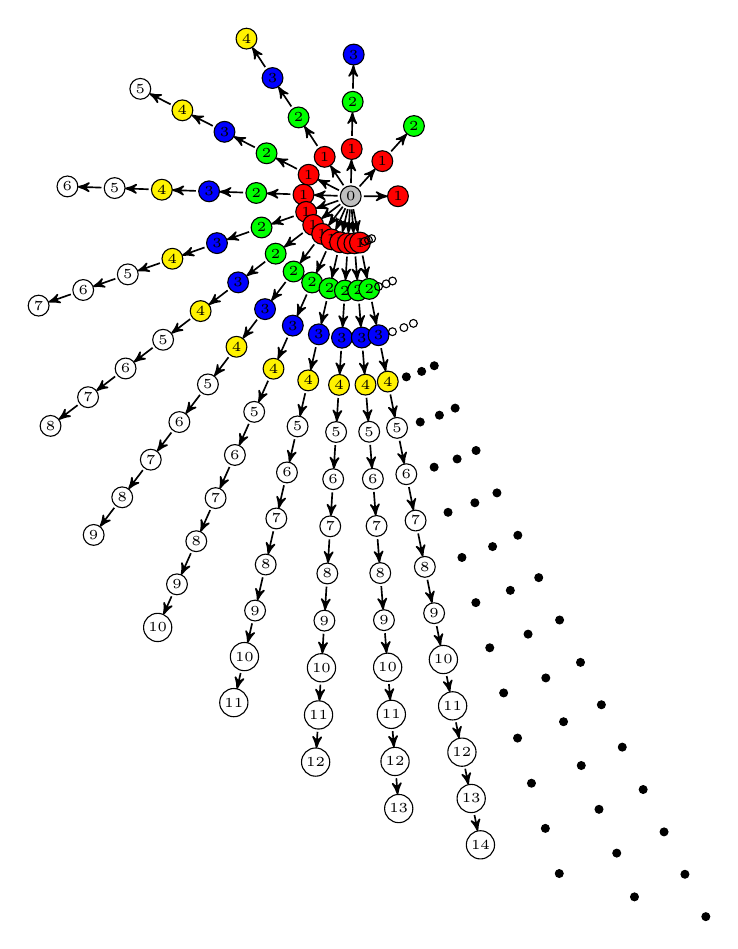
\begin{tikzpicture}[scale = 6]
\tikzstyle{VertexStyle}=[
shape = circle, 
minimum size = 1pt,
inner sep = 1pt,
draw]
\Vertex[style = {fill = lightgray, minimum size = 14pt}, x = 0.5, y = 0.5, L = \tiny {0}]{v0}
\Vertex[style = {fill = red, minimum size = 1pt}, x = 0.6, y = 0.5, L = \tiny {1}]{v1}
\Vertex[style = {fill = red, minimum size = 1pt}, x = 0.566913060635886, y = 0.574314482547739, L = \tiny {1}]{v2}
\Vertex[style = {fill = green, minimum size = 1pt}, x = 0.633826121271772, y = 0.648628965095479, L = \tiny {2}]{v3}
\Vertex[style = {fill = red, minimum size = 1pt}, x = 0.502094241988336, y = 0.599978068347485, L = \tiny {1}]{v4}
\Vertex[style = {fill = green, minimum size = 1pt}, x = 0.504188483976671, y = 0.699956136694969, L = \tiny {2}]{v5}
\Vertex[style = {fill = blue, minimum size = 1pt}, x = 0.506282725965007, y = 0.799934205042454, L = \tiny {3}]{v6}
\Vertex[style = {fill = red, minimum size = 1pt}, x = 0.444835412937157, y = 0.583407843361317, L = \tiny {1}]{v7}
\Vertex[style = {fill = green, minimum size = 1pt}, x = 0.389670825874314, y = 0.666815686722634, L = \tiny {2}]{v8}
\Vertex[style = {fill = blue, minimum size = 1pt}, x = 0.334506238811471, y = 0.750223530083951, L = \tiny {3}]{v9}
\Vertex[style = {fill = yellow, minimum size = 1pt}, x = 0.279341651748628, y = 0.833631373445269, L = \tiny {4}]{v10}
\Vertex[style = {fill = red, minimum size = 1pt}, x = 0.410932650758854, y = 0.545464351960143, L = \tiny {1}]{v11}
\Vertex[style = {fill = green, minimum size = 1pt}, x = 0.321865301517708, y = 0.590928703920286, L = \tiny {2}]{v12}
\Vertex[style = {fill = blue, minimum size = 1pt}, x = 0.232797952276562, y = 0.636393055880428, L = \tiny {3}]{v13}
\Vertex[style = {fill = yellow, minimum size = 1pt}, x = 0.143730603035416, y = 0.681857407840571, L = \tiny {4}]{v14}
\Vertex[style = {minimum size = 1pt}, x = 0.0546632537942704, y = 0.727321759800714, L = \tiny {5}]{v15}
\Vertex[style = {fill = red, minimum size = 1pt}, x = 0.400060049381855, y = 0.503465006557375, L = \tiny {1}]{v16}
\Vertex[style = {fill = green, minimum size = 1pt}, x = 0.300120098763709, y = 0.50693001311475, L = \tiny {2}]{v17}
\Vertex[style = {fill = blue, minimum size = 1pt}, x = 0.200180148145564, y = 0.510395019672125, L = \tiny {3}]{v18}
\Vertex[style = {fill = yellow, minimum size = 1pt}, x = 0.100240197527418, y = 0.513860026229501, L = \tiny {4}]{v19}
\Vertex[style = {minimum size = 1pt}, x = 0.000300246909272828, y = 0.517325032786876, L = \tiny {5}]{v20}
\Vertex[style = {minimum size = 1pt}, x = -0.0996397037088725, y = 0.520790039344251, L = \tiny {6}]{v21}
\Vertex[style = {fill = red, minimum size = 1pt}, x = 0.405626918655433, y = 0.46692853922894, L = \tiny {1}]{v22}
\Vertex[style = {fill = green, minimum size = 1pt}, x = 0.311253837310866, y = 0.43385707845788, L = \tiny {2}]{v23}
\Vertex[style = {fill = blue, minimum size = 1pt}, x = 0.216880755966299, y = 0.40078561768682, L = \tiny {3}]{v24}
\Vertex[style = {fill = yellow, minimum size = 1pt}, x = 0.122507674621732, y = 0.36771415691576, L = \tiny {4}]{v25}
\Vertex[style = {minimum size = 1pt}, x = 0.0281345932771656, y = 0.3346426961447, L = \tiny {5}]{v26}
\Vertex[style = {minimum size = 1pt}, x = -0.0662384880674013, y = 0.30157123537364, L = \tiny {6}]{v27}
\Vertex[style = {minimum size = 1pt}, x = -0.160611569411968, y = 0.26849977460258, L = \tiny {7}]{v28}
\Vertex[style = {fill = red, minimum size = 1pt}, x = 0.420574793531228, y = 0.439241160499949, L = \tiny {1}]{v29}
\Vertex[style = {fill = green, minimum size = 1pt}, x = 0.341149587062456, y = 0.378482320999898, L = \tiny {2}]{v30}
\Vertex[style = {fill = blue, minimum size = 1pt}, x = 0.261724380593685, y = 0.317723481499847, L = \tiny {3}]{v31}
\Vertex[style = {fill = yellow, minimum size = 1pt}, x = 0.182299174124913, y = 0.256964641999795, L = \tiny {4}]{v32}
\Vertex[style = {minimum size = 1pt}, x = 0.102873967656141, y = 0.196205802499744, L = \tiny {5}]{v33}
\Vertex[style = {minimum size = 1pt}, x = 0.0234487611873694, y = 0.135446962999693, L = \tiny {6}]{v34}
\Vertex[style = {minimum size = 1pt}, x = -0.0559764452814023, y = 0.0746881234996419, L = \tiny {7}]{v35}
\Vertex[style = {minimum size = 1pt}, x = -0.135401651750174, y = 0.0139292839995908, L = \tiny {8}]{v36}
\Vertex[style = {fill = red, minimum size = 1pt}, x = 0.439544303688558, y = 0.420343808881552, L = \tiny {1}]{v37}
\Vertex[style = {fill = green, minimum size = 1pt}, x = 0.379088607377116, y = 0.340687617763105, L = \tiny {2}]{v38}
\Vertex[style = {fill = blue, minimum size = 1pt}, x = 0.318632911065673, y = 0.261031426644657, L = \tiny {3}]{v39}
\Vertex[style = {fill = yellow, minimum size = 1pt}, x = 0.258177214754231, y = 0.181375235526209, L = \tiny {4}]{v40}
\Vertex[style = {minimum size = 1pt}, x = 0.197721518442789, y = 0.101719044407761, L = \tiny {5}]{v41}
\Vertex[style = {minimum size = 1pt}, x = 0.137265822131347, y = 0.0220628532893137, L = \tiny {6}]{v42}
\Vertex[style = {minimum size = 1pt}, x = 0.0768101258199045, y = -0.057593337829134, L = \tiny {7}]{v43}
\Vertex[style = {minimum size = 1pt}, x = 0.0163544295084623, y = -0.137249528947582, L = \tiny {8}]{v44}
\Vertex[style = {minimum size = 1pt}, x = -0.0441012668029799, y = -0.216905720066029, L = \tiny {9}]{v45}
\Vertex[style = {fill = red, minimum size = 1pt}, x = 0.459139197894626, y = 0.40872900323046, L = \tiny {1}]{v46}
\Vertex[style = {fill = green, minimum size = 1pt}, x = 0.418278395789251, y = 0.317458006460919, L = \tiny {2}]{v47}
\Vertex[style = {fill = blue, minimum size = 1pt}, x = 0.377417593683877, y = 0.226187009691379, L = \tiny {3}]{v48}
\Vertex[style = {fill = yellow, minimum size = 1pt}, x = 0.336556791578503, y = 0.134916012921839, L = \tiny {4}]{v49}
\Vertex[style = {minimum size = 1pt}, x = 0.295695989473129, y = 0.0436450161522983, L = \tiny {5}]{v50}
\Vertex[style = {minimum size = 1pt}, x = 0.254835187367754, y = -0.047625980617242, L = \tiny {6}]{v51}
\Vertex[style = {minimum size = 1pt}, x = 0.21397438526238, y = -0.138896977386782, L = \tiny {7}]{v52}
\Vertex[style = {minimum size = 1pt}, x = 0.173113583157006, y = -0.230167974156323, L = \tiny {8}]{v53}
\Vertex[style = {minimum size = 1pt}, x = 0.132252781051632, y = -0.321438970925863, L = \tiny {9}]{v54}
\Vertex[style = {minimum size = 1pt}, x = 0.0913919789462574, y = -0.412709967695403, L = \tiny {10}]{v55}
\Vertex[style = {fill = red, minimum size = 1pt}, x = 0.477505218718099, y = 0.402562918685547, L = \tiny {1}]{v56}
\Vertex[style = {fill = green, minimum size = 1pt}, x = 0.455010437436198, y = 0.305125837371093, L = \tiny {2}]{v57}
\Vertex[style = {fill = blue, minimum size = 1pt}, x = 0.432515656154296, y = 0.207688756056639, L = \tiny {3}]{v58}
\Vertex[style = {fill = yellow, minimum size = 1pt}, x = 0.410020874872395, y = 0.110251674742186, L = \tiny {4}]{v59}
\Vertex[style = {minimum size = 1pt}, x = 0.387526093590494, y = 0.0128145934277324, L = \tiny {5}]{v60}
\Vertex[style = {minimum size = 1pt}, x = 0.365031312308593, y = -0.084622487886721, L = \tiny {6}]{v61}
\Vertex[style = {minimum size = 1pt}, x = 0.342536531026691, y = -0.182059569201174, L = \tiny {7}]{v62}
\Vertex[style = {minimum size = 1pt}, x = 0.32004174974479, y = -0.279496650515628, L = \tiny {8}]{v63}
\Vertex[style = {minimum size = 1pt}, x = 0.297546968462889, y = -0.376933731830082, L = \tiny {9}]{v64}
\Vertex[style = {minimum size = 1pt}, x = 0.275052187180988, y = -0.474370813144535, L = \tiny {10}]{v65}
\Vertex[style = {minimum size = 1pt}, x = 0.252557405899086, y = -0.571807894458988, L = \tiny {11}]{v66}
\Vertex[style = {fill = red, minimum size = 1pt}, x = 0.49380832692355, y = 0.400191868144352, L = \tiny {1}]{v67}
\Vertex[style = {fill = green, minimum size = 1pt}, x = 0.487616653847101, y = 0.300383736288704, L = \tiny {2}]{v68}
\Vertex[style = {fill = blue, minimum size = 1pt}, x = 0.481424980770651, y = 0.200575604433057, L = \tiny {3}]{v69}
\Vertex[style = {fill = yellow, minimum size = 1pt}, x = 0.475233307694202, y = 0.100767472577409, L = \tiny {4}]{v70}
\Vertex[style = {minimum size = 1pt}, x = 0.469041634617752, y = 0.000959340721761182, L = \tiny {5}]{v71}
\Vertex[style = {minimum size = 1pt}, x = 0.462849961541303, y = -0.0988487911338866, L = \tiny {6}]{v72}
\Vertex[style = {minimum size = 1pt}, x = 0.456658288464853, y = -0.198656922989534, L = \tiny {7}]{v73}
\Vertex[style = {minimum size = 1pt}, x = 0.450466615388404, y = -0.298465054845182, L = \tiny {8}]{v74}
\Vertex[style = {minimum size = 1pt}, x = 0.444274942311954, y = -0.39827318670083, L = \tiny {9}]{v75}
\Vertex[style = {minimum size = 1pt}, x = 0.438083269235505, y = -0.498081318556478, L = \tiny {10}]{v76}
\Vertex[style = {minimum size = 1pt}, x = 0.431891596159055, y = -0.597889450412125, L = \tiny {11}]{v77}
\Vertex[style = {minimum size = 1pt}, x = 0.425699923082606, y = -0.697697582267773, L = \tiny {12}]{v78}
\Vertex[style = {fill = red, minimum size = 1pt}, x = 0.507815699725342, y = 0.400305893665657, L = \tiny {1}]{v79}
\Vertex[style = {fill = green, minimum size = 1pt}, x = 0.515631399450684, y = 0.300611787331314, L = \tiny {2}]{v80}
\Vertex[style = {fill = blue, minimum size = 1pt}, x = 0.523447099176027, y = 0.200917680996971, L = \tiny {3}]{v81}
\Vertex[style = {fill = yellow, minimum size = 1pt}, x = 0.531262798901369, y = 0.101223574662628, L = \tiny {4}]{v82}
\Vertex[style = {minimum size = 1pt}, x = 0.539078498626711, y = 0.0015294683282851, L = \tiny {5}]{v83}
\Vertex[style = {minimum size = 1pt}, x = 0.546894198352053, y = -0.0981646380060579, L = \tiny {6}]{v84}
\Vertex[style = {minimum size = 1pt}, x = 0.554709898077396, y = -0.197858744340401, L = \tiny {7}]{v85}
\Vertex[style = {minimum size = 1pt}, x = 0.562525597802738, y = -0.297552850674744, L = \tiny {8}]{v86}
\Vertex[style = {minimum size = 1pt}, x = 0.57034129752808, y = -0.397246957009087, L = \tiny {9}]{v87}
\Vertex[style = {minimum size = 1pt}, x = 0.578156997253422, y = -0.49694106334343, L = \tiny {10}]{v88}
\Vertex[style = {minimum size = 1pt}, x = 0.585972696978765, y = -0.596635169677773, L = \tiny {11}]{v89}
\Vertex[style = {minimum size = 1pt}, x = 0.593788396704107, y = -0.696329276012116, L = \tiny {12}]{v90}
\Vertex[style = {minimum size = 1pt}, x = 0.601604096429449, y = -0.796023382346459, L = \tiny {13}]{v91}
\Vertex[style = {fill = red, minimum size = 1pt}, x = 0.519612143348388, y = 0.40194203839931, L = \tiny {1}]{v92}
\Vertex[style = {fill = green, minimum size = 1pt}, x = 0.539224286696775, y = 0.303884076798621, L = \tiny {2}]{v93}
\Vertex[style = {fill = blue, minimum size = 1pt}, x = 0.558836430045163, y = 0.205826115197931, L = \tiny {3}]{v94}
\Vertex[style = {fill = yellow, minimum size = 1pt}, x = 0.57844857339355, y = 0.107768153597242, L = \tiny {4}]{v95}
\Vertex[style = {minimum size = 1pt}, x = 0.598060716741938, y = 0.00971019199655249, L = \tiny {5}]{v96}
\Vertex[style = {minimum size = 1pt}, x = 0.617672860090326, y = -0.088347769604137, L = \tiny {6}]{v97}
\Vertex[style = {minimum size = 1pt}, x = 0.637285003438713, y = -0.186405731204827, L = \tiny {7}]{v98}
\Vertex[style = {minimum size = 1pt}, x = 0.656897146787101, y = -0.284463692805516, L = \tiny {8}]{v99}
\Vertex[style = {minimum size = 1pt}, x = 0.676509290135488, y = -0.382521654406205, L = \tiny {9}]{v100}
\Vertex[style = {minimum size = 1pt}, x = 0.696121433483876, y = -0.480579616006895, L = \tiny {10}]{v101}
\Vertex[style = {minimum size = 1pt}, x = 0.715733576832263, y = -0.578637577607585, L = \tiny {11}]{v102}
\Vertex[style = {minimum size = 1pt}, x = 0.735345720180651, y = -0.676695539208274, L = \tiny {12}]{v103}
\Vertex[style = {minimum size = 1pt}, x = 0.754957863529039, y = -0.774753500808964, L = \tiny {13}]{v104}
\Vertex[style = {minimum size = 1pt}, x = 0.774570006877426, y = -0.872811462409653, L = \tiny {14}]{v105}
\Vertex[style = {minimum size = 1pt, draw = none}, x = 0.529426895250985, y = 0.404427735007025, L = \tiny {}]{v106}
\Vertex[style = {minimum size = 1pt, draw = none}, x = 0.558853790501971, y = 0.308855470014049, L = \tiny {}]{v107}
\Vertex[style = {minimum size = 1pt, draw = none}, x = 0.588280685752956, y = 0.213283205021073, L = \tiny {}]{v108}
\Vertex[style = {fill = black, minimum size = 1pt}, x = 0.617707581003942, y = 0.117710940028098, L = \tiny {}]{v109}
\Vertex[style = {fill = black, minimum size = 1pt}, x = 0.647134476254927, y = 0.0221386750351225, L = \tiny {}]{v110}
\Vertex[style = {fill = black, minimum size = 1pt}, x = 0.676561371505913, y = -0.073433589957853, L = \tiny {}]{v111}
\Vertex[style = {fill = black, minimum size = 1pt}, x = 0.705988266756898, y = -0.169005854950829, L = \tiny {}]{v112}
\Vertex[style = {fill = black, minimum size = 1pt}, x = 0.735415162007883, y = -0.264578119943804, L = \tiny {}]{v113}
\Vertex[style = {fill = black, minimum size = 1pt}, x = 0.764842057258869, y = -0.36015038493678, L = \tiny {}]{v114}
\Vertex[style = {fill = black, minimum size = 1pt}, x = 0.794268952509854, y = -0.455722649929755, L = \tiny {}]{v115}
\Vertex[style = {fill = black, minimum size = 1pt}, x = 0.82369584776084, y = -0.55129491492273, L = \tiny {}]{v116}
\Vertex[style = {fill = black, minimum size = 1pt}, x = 0.853122743011825, y = -0.646867179915706, L = \tiny {}]{v117}
\Vertex[style = {fill = black, minimum size = 1pt}, x = 0.882549638262811, y = -0.742439444908682, L = \tiny {}]{v118}
\Vertex[style = {fill = black, minimum size = 1pt}, x = 0.911976533513796, y = -0.838011709901657, L = \tiny {}]{v119}
\Vertex[style = {fill = black, minimum size = 1pt}, x = 0.941403428764781, y = -0.933583974894633, L = \tiny {}]{v120}
\Vertex[style = {minimum size = 1pt, draw = none}, x = 0.537536137682269, y = 0.407312145521122, L = \tiny {}]{v121}
\Vertex[style = {minimum size = 1pt, draw = none}, x = 0.575072275364539, y = 0.314624291042243, L = \tiny {}]{v122}
\Vertex[style = {minimum size = 1pt, draw = none}, x = 0.612608413046808, y = 0.221936436563365, L = \tiny {}]{v123}
\Vertex[style = {fill = black, minimum size = 1pt}, x = 0.650144550729078, y = 0.129248582084487, L = \tiny {}]{v124}
\Vertex[style = {fill = black, minimum size = 1pt}, x = 0.687680688411347, y = 0.0365607276056087, L = \tiny {}]{v125}
\Vertex[style = {fill = black, minimum size = 1pt}, x = 0.725216826093617, y = -0.0561271268732695, L = \tiny {}]{v126}
\Vertex[style = {fill = black, minimum size = 1pt}, x = 0.762752963775886, y = -0.148814981352148, L = \tiny {}]{v127}
\Vertex[style = {fill = black, minimum size = 1pt}, x = 0.800289101458156, y = -0.241502835831026, L = \tiny {}]{v128}
\Vertex[style = {fill = black, minimum size = 1pt}, x = 0.837825239140425, y = -0.334190690309904, L = \tiny {}]{v129}
\Vertex[style = {fill = black, minimum size = 1pt}, x = 0.875361376822695, y = -0.426878544788782, L = \tiny {}]{v130}
\Vertex[style = {fill = black, minimum size = 1pt}, x = 0.912897514504964, y = -0.519566399267661, L = \tiny {}]{v131}
\Vertex[style = {fill = black, minimum size = 1pt}, x = 0.950433652187234, y = -0.612254253746539, L = \tiny {}]{v132}
\Vertex[style = {fill = black, minimum size = 1pt}, x = 0.987969789869503, y = -0.704942108225417, L = \tiny {}]{v133}
\Vertex[style = {fill = black, minimum size = 1pt}, x = 1.02550592755177, y = -0.797629962704296, L = \tiny {}]{v134}
\Vertex[style = {fill = black, minimum size = 1pt}, x = 1.06304206523404, y = -0.890317817183174, L = \tiny {}]{v135}
\Vertex[style = {fill = black, minimum size = 1pt}, x = 1.10057820291631, y = -0.983005671662052, L = \tiny {}]{v136}
\Vertex[style = {minimum size = 1pt, draw = none}, x = 0.544212670813799, y = 0.410304739592827, L = \tiny {}]{v137}
\Vertex[style = {minimum size = 1pt, draw = none}, x = 0.588425341627599, y = 0.320609479185654, L = \tiny {}]{v138}
\Vertex[style = {minimum size = 1pt, draw = none}, x = 0.632638012441398, y = 0.23091421877848, L = \tiny {}]{v139}
\Vertex[style = {fill = black, minimum size = 1pt}, x = 0.676850683255197, y = 0.141218958371307, L = \tiny {}]{v140}
\Vertex[style = {fill = black, minimum size = 1pt}, x = 0.721063354068997, y = 0.0515236979641338, L = \tiny {}]{v141}
\Vertex[style = {fill = black, minimum size = 1pt}, x = 0.765276024882796, y = -0.0381715624430394, L = \tiny {}]{v142}
\Vertex[style = {fill = black, minimum size = 1pt}, x = 0.809488695696595, y = -0.127866822850213, L = \tiny {}]{v143}
\Vertex[style = {fill = black, minimum size = 1pt}, x = 0.853701366510395, y = -0.217562083257386, L = \tiny {}]{v144}
\Vertex[style = {fill = black, minimum size = 1pt}, x = 0.897914037324194, y = -0.307257343664559, L = \tiny {}]{v145}
\Vertex[style = {fill = black, minimum size = 1pt}, x = 0.942126708137993, y = -0.396952604071732, L = \tiny {}]{v146}
\Vertex[style = {fill = black, minimum size = 1pt}, x = 0.986339378951792, y = -0.486647864478906, L = \tiny {}]{v147}
\Vertex[style = {fill = black, minimum size = 1pt}, x = 1.03055204976559, y = -0.576343124886079, L = \tiny {}]{v148}
\Vertex[style = {fill = black, minimum size = 1pt}, x = 1.07476472057939, y = -0.666038385293252, L = \tiny {}]{v149}
\Vertex[style = {fill = black, minimum size = 1pt}, x = 1.11897739139319, y = -0.755733645700426, L = \tiny {}]{v150}
\Vertex[style = {fill = black, minimum size = 1pt}, x = 1.16319006220699, y = -0.845428906107599, L = \tiny {}]{v151}
\Vertex[style = {fill = black, minimum size = 1pt}, x = 1.20740273302079, y = -0.935124166514772, L = \tiny {}]{v152}
\Vertex[style = {fill = black, minimum size = 1pt}, x = 1.25161540383459, y = -1.02481942692195, L = \tiny {}]{v153}
\Edge[style = {post}](v0)(v1)
\Edge[style = {post}](v0)(v2)
\Edge[style = {post}](v2)(v3)
\Edge[style = {post}](v0)(v4)
\Edge[style = {post}](v4)(v5)
\Edge[style = {post}](v5)(v6)
\Edge[style = {post}](v0)(v7)
\Edge[style = {post}](v7)(v8)
\Edge[style = {post}](v8)(v9)
\Edge[style = {post}](v9)(v10)
\Edge[style = {post}](v0)(v11)
\Edge[style = {post}](v11)(v12)
\Edge[style = {post}](v12)(v13)
\Edge[style = {post}](v13)(v14)
\Edge[style = {post}](v14)(v15)
\Edge[style = {post}](v0)(v16)
\Edge[style = {post}](v16)(v17)
\Edge[style = {post}](v17)(v18)
\Edge[style = {post}](v18)(v19)
\Edge[style = {post}](v19)(v20)
\Edge[style = {post}](v20)(v21)
\Edge[style = {post}](v0)(v22)
\Edge[style = {post}](v22)(v23)
\Edge[style = {post}](v23)(v24)
\Edge[style = {post}](v24)(v25)
\Edge[style = {post}](v25)(v26)
\Edge[style = {post}](v26)(v27)
\Edge[style = {post}](v27)(v28)
\Edge[style = {post}](v0)(v29)
\Edge[style = {post}](v29)(v30)
\Edge[style = {post}](v30)(v31)
\Edge[style = {post}](v31)(v32)
\Edge[style = {post}](v32)(v33)
\Edge[style = {post}](v33)(v34)
\Edge[style = {post}](v34)(v35)
\Edge[style = {post}](v35)(v36)
\Edge[style = {post}](v0)(v37)
\Edge[style = {post}](v37)(v38)
\Edge[style = {post}](v38)(v39)
\Edge[style = {post}](v39)(v40)
\Edge[style = {post}](v40)(v41)
\Edge[style = {post}](v41)(v42)
\Edge[style = {post}](v42)(v43)
\Edge[style = {post}](v43)(v44)
\Edge[style = {post}](v44)(v45)
\Edge[style = {post}](v0)(v46)
\Edge[style = {post}](v46)(v47)
\Edge[style = {post}](v47)(v48)
\Edge[style = {post}](v48)(v49)
\Edge[style = {post}](v49)(v50)
\Edge[style = {post}](v50)(v51)
\Edge[style = {post}](v51)(v52)
\Edge[style = {post}](v52)(v53)
\Edge[style = {post}](v53)(v54)
\Edge[style = {post}](v54)(v55)
\Edge[style = {post}](v0)(v56)
\Edge[style = {post}](v56)(v57)
\Edge[style = {post}](v57)(v58)
\Edge[style = {post}](v58)(v59)
\Edge[style = {post}](v59)(v60)
\Edge[style = {post}](v60)(v61)
\Edge[style = {post}](v61)(v62)
\Edge[style = {post}](v62)(v63)
\Edge[style = {post}](v63)(v64)
\Edge[style = {post}](v64)(v65)
\Edge[style = {post}](v65)(v66)
\Edge[style = {post}](v0)(v67)
\Edge[style = {post}](v67)(v68)
\Edge[style = {post}](v68)(v69)
\Edge[style = {post}](v69)(v70)
\Edge[style = {post}](v70)(v71)
\Edge[style = {post}](v71)(v72)
\Edge[style = {post}](v72)(v73)
\Edge[style = {post}](v73)(v74)
\Edge[style = {post}](v74)(v75)
\Edge[style = {post}](v75)(v76)
\Edge[style = {post}](v76)(v77)
\Edge[style = {post}](v77)(v78)
\Edge[style = {post}](v0)(v79)
\Edge[style = {post}](v79)(v80)
\Edge[style = {post}](v80)(v81)
\Edge[style = {post}](v81)(v82)
\Edge[style = {post}](v82)(v83)
\Edge[style = {post}](v83)(v84)
\Edge[style = {post}](v84)(v85)
\Edge[style = {post}](v85)(v86)
\Edge[style = {post}](v86)(v87)
\Edge[style = {post}](v87)(v88)
\Edge[style = {post}](v88)(v89)
\Edge[style = {post}](v89)(v90)
\Edge[style = {post}](v90)(v91)
\Edge[style = {post}](v0)(v92)
\Edge[style = {post}](v92)(v93)
\Edge[style = {post}](v93)(v94)
\Edge[style = {post}](v94)(v95)
\Edge[style = {post}](v95)(v96)
\Edge[style = {post}](v96)(v97)
\Edge[style = {post}](v97)(v98)
\Edge[style = {post}](v98)(v99)
\Edge[style = {post}](v99)(v100)
\Edge[style = {post}](v100)(v101)
\Edge[style = {post}](v101)(v102)
\Edge[style = {post}](v102)(v103)
\Edge[style = {post}](v103)(v104)
\Edge[style = {post}](v104)(v105)
\end{tikzpicture}
\caption{The black hole graph.}
\label{fig:BlackHole}
\end{figure}

His definition, however, only captures this idea if sentences are restricted to finite length. When we are dealing with sentences of infinite length, then there are sentences, which are Herzberger-groundless, but which don't involve cycles or infinite paths. To see this consider the sentences system $(\S,d)$, where $\S = \{Z, X^1_1, X^2_1, X^2_2, X^3_1, X^3_2, X^3_3, \dots\}$ and $d(Z) = \bigwedge_{i \geq 1} \bigwedge_{1 \leq j \leq i} X^i_j$ and for each $X^i_j$ with $1 \leq j < i$, $d(X^i_j) = X^i_{j+1}$. Here $Z$ is Herzberger-groundless since for every natural number $k$ there is a chain of references of length $k$ to the sentence name $X^k_k$, so for any $k$, $D^k(\alpha)$ is non-empty. But there are no cycles and every path emanating from $Z$ terminates at some $k$ (see Figure \ref{fig:BlackHole}).

\prg A more useful and appropriate definition of \textit{ungroundedness}, however, is close at hand. Let's first define a \textit{ray}, which is an infinite  set of vertices connected by an infinite chain of directed edges.

\begin{defn}
A \emph{ray} in a directed graph $G$ is a subgraph with vertex set $\{v_i\}_{i < \omega}$ and edge set $\{(v_i, v_{i + 1})\}_{i < \omega}$.
\end{defn}

%% ray %%
\begin{figure}[h]
\centering
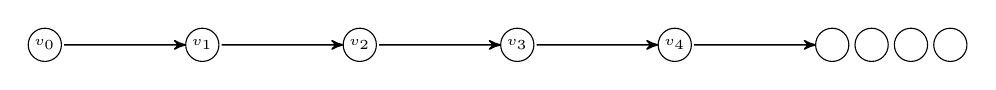
\begin{tikzpicture}[scale = 10]
\tikzstyle{VertexStyle}=[shape = circle,	
								 minimum size = 12 pt,
								 inner sep = 1.2pt,
                         draw]
\Vertex[x = 0.0, y = 0.5, L = \tiny {$v_0$}]{v0}
\Vertex[x = 0.2, y = 0.5, L = \tiny {$v_1$}]{v1}
\Vertex[x = 0.4, y = 0.5, L = \tiny {$v_2$}]{v2}
\Vertex[x = 0.6, y = 0.5, L = \tiny {$v_3$}]{v3}
\Vertex[x = 0.8, y = 0.5, L = \tiny {$v_4$}]{v4}
\Vertex[style = {draw = none}, x = 1.0, y = 0.5, L = \tiny {}]{v5}
\Vertex[style = {minimum size = 1 pt}, x = 1.05, y = 0.5, L = \tiny {}]{v6}
\Vertex[style = {minimum size = 1 pt}, x = 1.1, y = 0.5, L = \tiny {}]{v7}
\Vertex[style = {minimum size = 1 pt}, x = 1.15, y = 0.5, L = \tiny {}]{v8}
\Edge[style = {post}](v0)(v1)
\Edge[style = {post}](v1)(v2)
\Edge[style = {post}](v2)(v3)
\Edge[style = {post}](v3)(v4)
\Edge[style = {post}](v4)(v5)
\end{tikzpicture}
\caption{A ray.}
\label{fig:ray}
\end{figure}
%%

\begin{defn}
A directed graph $G$ is \emph{ungrounded} if it contains a ray or a directed cycle.  Otherwise $G$ is \emph{grounded}.\footnote{An anonymous referee suggests the following equivalent definition of ungrounded: a directed graph $G$ is \emph{ungrounded} if $G$ has a subgraph $H$ in which every vertex has positive out-degree.}
\end{defn}

Intuitively, if $G$ is grounded, then we can obtain an acceptable truth assignment for any denotation assignment on $V(G)$ by repeatedly substituting the values of constant sentences in for their names.  Since we don't make any arbitrary choices in this process, the constructed acceptable truth assignment should be unique.  To make performing this operation infinitely many times precise we will apply Zorn's lemma.  Later we will use a similar proof idea to prove a more general result.

\begin{zorn}
Every partially ordered set, in which every chain (i.e. totally ordered subset) has an upper bound, contains at least one maximal element.
\end{zorn}

\begin{defn}
Let $G$ be a directed graph.  We say that $A \subseteq V(G)$ is \emph{self-contained} in $G$ if there are no edges in $G$ directed from $A$ to $G - A$.  
\end{defn}

\begin{lem}\label{GroundedNotDangerous}
If a directed graph $G$ is grounded, then it is not dangerous and not precarious.
\end{lem}
\begin{proof}
Assume $G$ is grounded.  Let $d$ be a denotation assignment on $V(G)$ such that $G = \G_{V(G), d}$. We will show that there is a unique acceptable truth assignment on $V(G)$ with respect to $d$.  Since $d$ was arbitrary, it follows that $G$ is not dangerous and not precarious.

For $A \subseteq V(G)$ which is self-contained in $G$, let $d_A$ be $d$ restricted to $A$.  Then $d_A$ is a denotation assignment on $A$.  If $A$ has a unique acceptable truth assignment with respect to $d_A$, then we call this truth assignment $v_A$ and call the pair $(A, v_A)$ \emph{solved}.

Let $X$ be the collection of all solved pairs.  Define a partial order $<$ on $X$ by $(A, v_A) < (B, v_B)$ if and only if $A \subsetneq B$ and $v_A$ is $v_B$ restricted to $A$.

To apply Zorn's lemma to $(X, <)$, we need to show that $X \neq \emptyset$ and that every chain in  $(X, <)$ has an upper bound. Since $(\emptyset, v_\emptyset) \in X$ we see that $X \neq \emptyset$.  Now let $(A_1, v_{A_1}) < (A_2, v_{A_2}) < \cdots$ be an arbitrary chain in $(X, <)$.  Put $U = \bigcup_{i > 0} A_i$. Plainly, $U$ is self-contained in $G$. For $u \in U$, let $h(u)$ be the smallest $i > 0$ such that $u \in A_i$.  Now, for $u \in U$, let $v_U(u) = v_{A_{h(u)}}(u)$.  We claim that $(U, v_U)$ is an upper bound for the chain.  By definition $A_i \subseteq U$ and $v_{A_i}$ is $v_U$ restricted to $A_i$ for each $i > 0$.  It remains to be shown that $v_U$ is the unique acceptable truth assignment on $U$ with respect to $d_U$.  Assume $v_U$ is not acceptable and pick $u \in U$ with $h(u)$ minimal such that $v_U(u) \neq \llbracket d_U(u)\rrbracket(v_U)$.  Put $B = A_{h(u)}$. Then

\[v_B(u) = v_U(u) \neq \llbracket d_U(u)\rrbracket(v_U) = \llbracket d_B(u)\rrbracket(v_B) = v_B(u).\]

This is a contradiction.  Hence $v_U$ is acceptable.  To see that $v_U$ is unique, assume there is a different acceptable truth assignment on $U$ with respect to $d_U$, call it $v_O$.  Take $u \in U$ with $h(u)$ minimal such that $v_U(u) \neq v_O(u)$.  Again put $B = A_{h(u)}$.  Then $v_O$ restricted to $B$ is an acceptable truth assignment on $B$ with respect to $d_B$ which is different from $v_B$.  This is a contradiction.  Thus we conclude that $(U, v_U)$ is an upper bound for the chain.

Applying Zorn's lemma gives us a solved pair $(M, v_M)$ which is maximal in $(X, <)$.  We will show that $M = V(G)$ and hence $v_M$ is the desired unique acceptable truth assignment on $V(G)$ with respect to $d$.  So assume $M \neq V(G)$.  Put $J = V(G) - M$.

First assume that there is some $z \in J$ such that $T = M \cup \{z\}$ is self-contained.  Since $T$ is self-contained, $d(z)$ involves only elements of $M$.  Thus, letting $v_T(x) = v_M(x)$ for each $x \in M$ and $v_T(z) = d(z)[x \Rightarrow v_M(x) \mid x \in M]$ makes $v_T$ the unique acceptable truth assignment on $T$ with respect to $d_T$.  We conclude that $(T, v_T) \in X$ and $(M, v_M) < (T, v_T)$ contradicting the maximality of $(M, v_M)$.

Thus we may assume that $N^+(z) \cap J \neq \emptyset$ for each $z \in J$.  Pick $z_0 \in J$.  For $k > 0$, let $z_k \in N^+(z_{k - 1}) \cap J$.  Since $G$ is acyclic, $z_0z_1z_2\cdots$ is a ray in $G$ contradicting the fact that $G$ is grounded.  Whence $M = V(G)$ and the proof is complete.
\end{proof}

\begin{lem}\label{DirectedCyclesMakeDanger}
If a directed graph $G$ contains a directed cycle, then it is both dangerous and precarious.
\end{lem}
\begin{proof}
By Lemma \ref{SubgraphDangerLemma}, we can assume that $G$ is a directed cycle.  Let $V(G) = \{v_1, \ldots, v_k\}$.  Let $d$ be a denotation assignment on $V(G)$ with $d(v_i) = \neg v_{i + 1}$ for $i < k$, $d(v_k) = \neg v_1$ if $k$ is odd and $d(v_k) = v_1$ if $k$ is even.  Then $G = \G_{V(G), d}$ and $(V(G), d)$ is paradoxical.  Hence $G$ is dangerous.  To see that $G$ is precarious, just consider the denotation assignment $d'$ on $V(G)$ with $d'(v_i) = v_{i + 1}$ for $i < k$ and $d(v_k) = v_1$.  Both the truth assignment setting all the $v_i$ to $1$ and the truth assiggment setting all the $v_i$ to $0$ are acceptable.
\end{proof}

\begin{thm}\label{PrecariousCharacterization}
A directed graph $G$ is precarious if and only if it is ungrounded.
\end{thm}
\begin{proof}
Lemma \ref{GroundedNotDangerous} gives the forward implication.  For the reverse implication, by Lemma \ref{SubgraphDangerLemma} and Lemma \ref{DirectedCyclesMakeDanger} we only need to consider the case of $G$ being a ray with vertex set $\{v_i\}_{i < \omega}$.  Let $d$ be a denotation assignment on $V(G)$ with $d(v_i) = v_{i+1}$.  Then $G = \G_{V(G), d}$ and $(V(G), d)$ is hypodoxical because we get two acceptable truth-value assignments by setting all the $v_i$ to $1$ or setting all the $v_i$ to $0$.
\end{proof}

\begin{cor}
If a directed graph is dangerous then it is precarious.
\end{cor}

In the finite case, we get the following complete characterization of danger. 
\begin{cor}\label{FiniteCharacterization}
Let $G$ be a finite directed graph.  The following are equivalent:
\begin{itemize}
\item[(a)] $G$ is dangerous;
\item[(b)] $G$ is precarious;
\item[(c)] $G$ contains a directed cycle;
\item[(d)] $G$ contains a subdivision of the Liar graph.
\end{itemize}
\end{cor}

The results above exhaust the relations between ungroundedness, cyclicity, precarity and danger; that is, there are ungrounded graphs that are not dangerous (the ray in Figure \ref{fig:ray}), precarious graphs that are not dangerous (again the ray in Figure \ref{fig:ray}) and dangerous graphs that contain no cycle (the Yablo graph in Figure \ref{fig:yablo}).

\begin{defn}
A \emph{homomorphism} from a directed graph $G$ to a directed graph $H$ is a function $f:V(G) \rightarrow V(H)$ such that if $xy \in E(G)$, then $f(x)f(y) \in E(H)$.   If $f$ is a bijection, and $f^{-1}: V(H) \rightarrow V(G)$ is a homomorphism, the we call $f$ an \emph{isomorphism}.  Additionally, we call the graph with vertex set $f(V(G))$ and edge set $\{f(x)f(y) \mid xy \in E(G)\}$ the \emph{homomorphic image} of $G$ under $f$.
\end{defn}

In Figure \ref{fig:homomorphic} we see an example of a non-isomorphic homomorphic image.  Additionally, since a path of length one is neither precarious nor dangerous, this example shows that taking of a homomorphic image can introduce precarity and danger. However, precarity cannot be lost by
taking a homomorphic image as the next lemma shows.

% homomorphic image %

\begin{figure}[ht]
\centering
\subfloat[] {
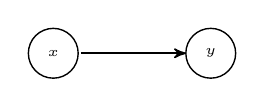
\begin{tikzpicture}[scale = 2]
\Vertex[x = 0.0, y = 0.0, L = \tiny {$x$}]{v0}
\Vertex[x = 1.0, y = 0.0, L = \tiny {$y$}]{v1}
\Edge[style = {post}](v0)(v1)
\end{tikzpicture}
}
\qquad
\subfloat[] {
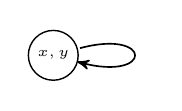
\begin{tikzpicture}[scale = 2]
\Vertex[x = 0.0, y = 0.0, L = \tiny {$x, y$}]{v0}
\Edge[style = {loop right, post}](v0)(v0)
\end{tikzpicture}
}
\caption{The Liar graph is a homomorphic image of the path of length one.}
\label{fig:homomorphic}
\end{figure}
%%

\begin{lem}
Let $G$ be a directed graph.  Then $G$ is precarious if and only if every homomorphic image of $G$ is precarious.
\end{lem}
\begin{proof}
Since $G$ is a homomorphic image of it self, the reverse implication is trivial.  To prove the forward implication, assume $G$ is precarious.  Then, by Theorem \ref{PrecariousCharacterization} $G$ contains a directed cycle or a ray.  Let $H$ be a homomorphic image of $G$ and let $f:V(G) \rightarrow V(H)$ be a homomorphism.  If there is a directed path between $x,y \in V(G)$, then we cannot have $f(x) = f(y)$, for otherwise $H$ would contain a directed cycle and hence be precarious.  In particular, $G$ cannot contain a directed cycle.  Thus $G$ contains a ray $\{v_i\}_{i < \omega}$.  If $f(v_i) = f(v_j)$ for $i \neq j$, then $H$ contains a directed cycle and we are done.  Otherwise $H$ contains a ray and we are done.
\end{proof}

\begin{conj}
Let $G$ be a directed graph.  Then $G$ is dangerous if and only if every homomorphic image of $G$ is dangerous.
\end{conj}

\section{Compactness and dangerous tails}
\label{sec6}

\subsection{Locally finite graphs}
Using the compactness theorem of first-order logic, we will show that graphs for which $N^+(v)$ is finite for every vertex $v$ are not dangerous. 

\begin{compactness}
A set of first-order sentences has a model if and only if every finite subset of it has a model.
\end{compactness}

To apply this theorem we need to be careful since a first-order sentence must have finite length. The following generalization of Lemma \ref{LanguageIsCompleteSimple} gives us the control over the lengths of sentences that we need.

\begin{defn}
For $v \in \V_\S$ and $I \subseteq \S$, let
\[v^I = \left\{u \in  \V_\S \mid \forall_{\alpha \in \S - I} u(\alpha) = v(\alpha)\right\}.\]
\end{defn}

\begin{defn}
Let $g$ be a function from $\V_\S$ to $\{0, 1\}$.  We say that $g$ is \emph{independent of} $I \subseteq \S$ if $g$ is constant on $v^I$ for each $v \in \V_\S$.
\end{defn}

Note that every such function is independent of the empty set.

\begin{lem}\label{LanguageIsComplete}
For any function $g$ from $\V_\S$ to $\{0, 1\}$ and any $I \subseteq \S$ of which $g$ is independent, there exists a sentence $\zeta_{g, I} \in \S^+$ with the following properties:
\begin{itemize}
\item $\;\;$ no sentence name from $I$ appears in $\zeta_{g, I}$;  
\item $\;\;$ $\zeta_{g, I} = g$;
\item $\;\;$ $\zeta_{g, I}$ has finite length if $\S - I$ is finite.
\end{itemize}
\end{lem}

\begin{proof}
Let $g$ be a function from $\V_\S$ to  $\{0, 1\}$.  First, if $g$ is a constant function, put $\zeta_{g, I} = \top$ if $g$ maps everything to $1$ and $\zeta_{g, I} = \bot$ if $g$ maps everything to $0$.

Otherwise $\S - I$ has at least one element and we proceed as follows.  Let $B = \{v \in \V_\S \mid \forall_{\alpha \in I} v(\alpha) = 0\}$. Note that $g$ is completely determined by its values on the elements of $B$.

For $v \in \V_\S$ and $\alpha \in \S$, let 

\[P(v, \alpha) = \begin{cases}
\alpha & \text{if } v(\alpha) = 1 \\
\neg \alpha & \text{if } v(\alpha) = 0
\end{cases}.\]

Let $C = \{v \in B \mid g(v) = 1 \}$. For $v \in C$, define

\[\chi_v = \bigwedge_{\alpha \in \S - I} P(v, \alpha).\] 

Note that $\chi_v(r) = g(r)$ if $r = v$ and $\chi_v(r) = 0$ if $r \neq v$. Let $\zeta_{g, I}$ be the sentence
\[\bigvee_{v \in C} \chi_v.\]

Then, for any $r \in \V_\S$, we have 

\[\llbracket \zeta_{g, I} \rrbracket(r) = \left\llbracket\bigvee_{v \in C} \chi_v \right\rrbracket(r) = \bigvee_{v \in C} \llbracket \chi_v \rrbracket(r) = \llbracket \chi_r \rrbracket(r) = g(r).\]

Hence $\zeta_{g, I} = g$.  Now the length of  $\zeta_{g, I}$ is at most $|C||\S - I| \leq |B||\S - I| \leq 2^{|\S - I|}|\S - I|$. Thus $\zeta_{g, I}$ has finite length if  $\S - I$ is finite. 
\end{proof}

\begin{lem}\label{LocalFinite}
Let $G$ be a directed graph such that $|N^{+}_G(v)|$ is finite for every $v \in V(G)$.  If $G$ is dangerous then some finite subraph of $G$ is dangerous.
\end{lem}
\begin{proof}
Assume that no finite subgraph of $G$ is dangerous and let $d$ be a denotation assignment on $V(G)$ such that $G = \G_{V(G), d}$.  For each $v \in V(G)$, put $I_v = V(G) - N^+_G(v)$. Construct a first order language $\fancy{L}$ as follows.  The constants of $\L$ are the vertices of $G$ together with $\top$ and $\bot$.  The axioms are the following.

\begin{itemize}
\item $\;\;$ $\top \neq \bot$
\item $\;\;$ $x = \top \vee x = \bot$ for each $x \in V(G)$,
\item $\;\;$ $x = \zeta_{\llbracket d(x) \rrbracket, I_x}$ for each $x \in V(G)$.
\end{itemize}

By Lemma \ref{LanguageIsComplete} each of the sentences is of finite length.  Note that a model of the language is an acceptable truth assignment on $V(G)$ relative to $d$.  Since no finite subgraph of $G$ is dangerous, every finite subset of the axioms has a model.  Thus, by compactness, the whole language has a model and hence $(V(G), d)$ is not paradoxical.  Since $d$ was arbitrary, we conclude that $G$ is not dangerous.\footnote{The proof technique used here is very similar to the compactness-based proof of the De Bruijn-Erd{\"o}s coloring theorem (\cite{erdos51}) stating that an infinite graph can be $k$-colored if and only if each of its finite subgraphs can be $k$-colored.  Lemma \ref{LocalFinite} can also be proved (as can the De Bruijn-Erd{\"o}s theorem) by directly applying Zorn's lemma as we need to do in the more complicated results below.}
\end{proof}

\begin{cor}\label{AtLeastOneInfinite}
Any directed acyclic graph $G$ such that $|N^{+}_G(v)|$ is finite for every $v \in V(G)$ is not dangerous.
\end{cor}
\begin{proof}
Combine Corollary \ref{FiniteCharacterization} and Lemma \ref{LocalFinite}.
\end{proof}

\subsection{Topological sorting}

Now we show that if $G$ is an acyclic directed graph then its vertices can be ordered left to right such that edges only go to the right.  

\begin{defn}
Let $G$ be a directed graph.  A vertex $v \in V(G)$ is called a \emph{sink} if $N^+_G(v)$ is empty and a \emph{source} if $N^-_G(v)$ is empty.
\end{defn}

%% sinks & sources %%
\begin{figure}[h]
\centering
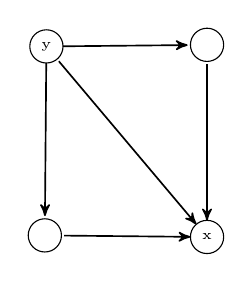
\begin{tikzpicture}[scale = 10]
\tikzstyle{VertexStyle}=[shape = circle,	
								 minimum size = 12pt,
								 inner sep = 1.2pt,
                         draw]
\Vertex[x = 0.605999946594238, y = 0.470000028610229, L = \tiny {x}]{v0}
\Vertex[x = 0.401999980211258, y = 0.712000012397766, L = \tiny {y}]{v1}
\Vertex[x = 0.606000065803528, y = 0.71399998664856, L = \tiny {}]{v2}
\Vertex[x = 0.400000005960464, y = 0.472000002861023, L = \tiny {}]{v3}
\Edge[style = {post}](v1)(v0)
\Edge[style = {pre}](v2)(v1)
\Edge[style = {post}](v2)(v0)
\Edge[style = {pre}](v3)(v1)
\Edge[style = {post}](v3)(v0)
\end{tikzpicture}
\caption{A graph with sink $x$ and source $y$.}
\end{figure}
%%

\begin{defn}
Let $G$ be a directed graph.  A \emph{topological sort} on $G$ is a total ordering $<$ of $V(G)$ such that if $(a,b) \in E(G)$, then $a < b$.
\end{defn}

We prove the following easy lemma for completeness.
\begin{lem}
If $G$ is a finite directed acyclic graph, then $G$ has a topological sort.
\end{lem}
\begin{proof}
Assume (to reach a contradiction) that the lemma is false and let $G$ be a counterexample with the minimum number of vertices.  Since $G$ is finite it has a source $v$.  By minimality $G - v$ has a topological sort $\{v_1, \ldots, v_r\}$.  But then $\{v, v_1, \ldots, v_r\}$ is a topological sort of $G$. This is a contradiction.
\end{proof}

\begin{lem}\label{TopSortExists}
Let $G$ be an directed acyclic graph. Then $G$ has a topological sort.
\end{lem}
\begin{proof}
We construct a first order language $\fancy{L}$ and apply the compactness theorem.  Let the elements of $V(G)$ be the constants of $\fancy{L}$ and let $R$ be $\fancy{L}$'s only relation symbol.  Define the axioms of $\fancy{L}$ as follows.

\begin{itemize}
\item $\;\;$ $\neg (a = b)$ for all distinct $a,b \in V(G)$,
\item $\;\;$ $aRb$ for all $(a,b) \in E(G)$,
\item $\;\;$ $aRb \rightarrow \neg (bRa)$ for all $a,b \in V(G)$,
\item $\;\;$ $aRb \vee bRa \vee a = b$ for all $a,b \in V(G)$,
\item $\;\;$ $(aRb \wedge bRc) \rightarrow aRc$ for all $a,b,c \in V(G)$.
\end{itemize}

Let $A$ be a finite subset of the axioms.  Let $C$ be the set of all constants appearing in some axiom of $A$.  Create $A'$ from $A$ by adding in all axioms involving only the elements of $C$.  Then $A'$ is still finite and if $A'$ has a model, so does $A$.  Put $H = G[C]$.  Since $H$ is finite and acyclic it has a topological sort $<$.  Letting $<$ be the interpretation of $R$ gives a model of $A'$ and hence $A$.

Thus, by the compactness theorem, the entire set of axioms has a model.  The interpretation of $R$ in this model is the desired topological sort.
\end{proof}

\subsection{Dangerous tails}
\begin{lem}\label{GeneralZorn}
Let $G$ be a directed graph. If for every induced subgraph $H$ of $G$ there exists $\emptyset \neq C \subseteq V(H)$ which is self-contained in $H$ such that $G[C]$ is not dangerous, then $G$ is not dangerous.
\end{lem}
\begin{proof}
Assume that for every induced subgraph $H$ of $G$ there exists $\emptyset \neq C \subseteq V(H)$ which is self-contained in $H$ such that $G[C]$ is not dangerous.  Let $d$ be a denotation assignment on $V(G)$ such that $G = \G_{V(G), d}$. We will show that there is an acceptable truth assignment on $V(G)$ with respect to $d$.  Since $d$ was arbitrary, it follows that $G$ is not dangerous.

For $A \subseteq V(G)$ which is self-contained in $G$, let $d_A$ be $d$ restricted to $A$.  Then $d_A$ is a denotation assignment on $A$.  If $A$ has an  acceptable truth assignment with respect to $d_A$, then we pick an acceptable truth assignment $v_A$ and call the pair $(A, v_A)$ \emph{solved}.

Let $X$ be the collection of all solved pairs.  Define a partial order $<$ on $X$ by $(A, v_A) < (B, v_B)$ if and only if $A \subsetneq B$ and $v_A$ is $v_B$ restricted to $A$.

To apply Zorn's lemma to $(X, <)$, we need to show that $X \neq \emptyset$ and that every chain in  $(X, <)$ has an upper bound. Since $(\emptyset, v_\emptyset) \in X$ we see that $X \neq \emptyset$.  Now let $(A_1, v_{A_1}) < (A_2, v_{A_2}) < \cdots$ be an arbitrary chain in $(X, <)$.  Put $U = \bigcup_{i > 0} A_i$. Plainly, $U$ is self-contained in $G$. For $u \in U$, let $h(u)$ be the smallest $i > 0$ such that $u \in A_i$.  Now, for $u \in U$, let $v_U(u) = v_{A_{h(u)}}(u)$.  We claim that $(U, v_U)$ is an upper bound for the chain.  By definition $A_i \subseteq U$ and $v_{A_i}$ is $v_U$ restricted to $A_i$ for each $i > 0$.  It remains to be shown that $v_U$ is an acceptable truth assignment on $U$ with respect to $d_U$.  Assume $v_U$ is not acceptable and pick $u \in U$ with $h(u)$ minimal such that $v_U(u) \neq \llbracket d_U(u)\rrbracket(v_U)$.  Put $B = A_{h(u)}$. Then

\[v_B(u) = v_U(u) \neq \llbracket d_U(u)\rrbracket(v_U) = \llbracket d_B(u)\rrbracket(v_B) = v_B(u).\]

This is a contradiction.  Hence $v_U$ is acceptable.  Thus we conclude that $(U, v_U)$ is an upper bound for the chain.

Applying Zorn's lemma gives us a solved pair $(M, v_M)$ which is maximal in $(X, <)$.  We will show that $M = V(G)$ and hence $v_M$ is the desired acceptable truth assignment on $V(G)$ with respect to $d$.  So assume $M \neq V(G)$.  Put $H = G - M$.  By assumption, we have $\emptyset \neq C \subseteq V(H)$ which is self-contained in $H$ such that $G[C]$ is not dangerous.  Put $B = M \cup C$.  Note that $B$ is self-contained.  Since $C$ is not dangerous, we can extend $v_M$ to an acceptable truth assignment $v_B$ on $B$ with respect to $d_B$.  But then $(B, v_B) \in X$ and $(B, v_B) > (M, v_M)$ contradicting the maximality of $(M, v_M)$. Hence $M = V(G)$ and the proof is complete.
\end{proof}


A good way to get self-contained sets in an acyclic graph is to topological sort the graph and take all vertices ``to the right'' of a given vertex.  To make this precise we introduce the concept of a tail.

\begin{defn}
Let $G$ be a directed acyclic graph and let $<$ be a topological sort on $G$.  For $z \in V(G)$, the $z$-tail of $G$ (with respect to $<$) is the subgraph induced on $\{x \in V(G) \mid x > z\}$.  An induced subgraph of $G$ that is a $z$-tail for some $z \in V(G)$ is called a \emph{tail} of $G$.
\end{defn}

\begin{lem}\label{TailLemma}
Let $G$ be a directed acyclic graph and let $<$ be a topological sort on $G$.  If every induced subgraph of $G$ has a tail which is not dangerous, then $G$ is not dangerous.
\end{lem}
\begin{proof}
Let $H$ be an arbitrary induced subgraph of $G$.  We need to show that there exists $\emptyset \neq A \subseteq V(H)$ which is self-contained in $H$ such that $G[A]$ is not dangerous.  Pick $z \in V(H)$ such that the $z$-tail of $H$ is not dangerous.  Let $T_z$ be the $z$-tail of $H$.  Note that $T_z$ is self-contained.  Thus, if $T_z$ is non-empty, then we are done.  Hence we may assume that $T_z$ is empty.  But then $x \leq z$ for every $x \in V(H)$.  Hence $z$ is a sink in H and in particular, $\{z\}$ is a non-empty, self-contained set which induces a non-dangerous graph.  This completes the proof.
\end{proof}

\begin{cor}\label{InfinitelyManyInfinite}
If $G$ is a dangerous directed acyclic graph, then $|N^{+}_G(v)|$ is infinite for infinitely many $v \in V(G)$.
\end{cor}
\begin{proof}
Let $G$ be a directed acyclic graph $G$ such that $|N^{+}_G(v)|$ is infinite for only finitely many $v \in V(G)$.  By Lemma \ref{TopSortExists} $G$ has a topological sort $<$.  Let $H$ be an arbitrary induced subgraph of $G$. Since there are only finitely many $v \in V(H)$ with $|N^{+}_G(v)|$ infinite, there is a largest (under the order $<$) such vertex $z_H$.  Then the $z_H$-tail of $H$ has no vertices with infinite out degree and hence is not dangerous by Lemma \ref{LocalFinite}.  Thus every induced subgraph of $G$ has a non-dangerous tail.  Applying Lemma \ref{TailLemma} finishes the proof.
\end{proof}

\section{Reciprocity and underlying graphs}
\label{recip}
Let $\S = \{A_1, A_2, \ldots\}$ and $d(A_i) = \neg A_{i+1}$.  Then the reference graph of the sentence system $(\S, d)$ is the ray and we know that this is precarious but not dangerous from above.  Intuitively, in the reference graph we have an edge from $A_1$ to $A_2$ because $d(A_1)$ is ``a function of'' of $A_2$.\footnote{This intuitive idea of ``dependence" can only be taken so far. In Appendix \ref{dependence} we show that defining a graph based on ``dependence'' turns out to be useless in general.} In this case, fixing the value of $A_2$ determines what the value of $A_1$ must be.  But it is also true that fixing the value of $A_1$ determines what the value of $A_2$ must be---so $A_1$ and $A_2$ are reciprocal. Looking at it this way, we would want to see an edge going in both directions.  We can capture these intuitive ideas by considering necessary and sufficient conditions for danger on the underlying \textit{undirected} graph of a directed graph $G$.

\begin{defn}
Let $G$ be a directed graph.  The \emph{underlying undirected graph} of $G$ is the graph $\U(G)$ with vertex set $V(G)$ and an edge between $x, y \in V(G)$ for each $xy \in E(G)$ and $yx \in E(G)$.  We also call $G$ an \emph{orientation} of $\U(G)$.\footnote{Note that if $G$ contains a cycle of length two through vertices $x$ and $y$---such as in Jourdain's paradox---then $\U(G)$ will have two edges between $x$ and $y$.}
\end{defn}

It turns out that we can completely classify the undirected graphs which have dangerous orientations---they are precisely the ones containing a cycle.

\begin{thm}\label{OrientationDangerous}
A graph has a dangerous orientation if and only if it contains a cycle.
\end{thm}
\begin{proof}
The reverse direction is easy, since if $F$ is a graph that contains a cycle we may orient the edges of the cycle clockwise and the other edges arbitrarily and conclude that the orientation is dangerous using Lemma \ref{DirectedCyclesMakeDanger}.

For the forward direction, assume $G$ is a directed graph such that $\U(G)$ is acyclic. Let $d$ be a denotation assignment on $V(G)$ such that $G = \G_{V(G), d}$.  By Lemma \ref{JunkRemoval} we may assume that there is no ``junk''; that is, for every $x \in V(G)$, if $d(x) \not \in \{\bot, \top\}$, then there exist truth assignments $v_0, v_1$ on $V(G)$ such that $\llbracket d(x)\rrbracket(v_0) = 0$ and  $\llbracket d(x)\rrbracket(v_1) = 1$.   Also, without loss of generality, we may assume that $\U(G)$ is connected.

For $A \subseteq V(G)$, call $x \in A$ \emph{interior} to $A$ if $x$ has no edges to $G - A$.  The set of interior vertices of $A$ is the \emph{interior} of $A$ and is denoted $\I(A)$. Let the \emph{exterior} vertices of $A$ be $\E(A) = A - \I(A)$.  Call $A \subseteq V(G)$ \emph{tame} if $\U(G[A])$ is connected and for each $x \in \E(A)$ we have $N^+(x) \cap A = \emptyset$. Additionally, let $d_A$ be $d$ restricted to $A$.  We need to extend the notion of acceptable truth assignment as follows.  A function $v$ from $A$ to $\{0,1\}$ is called acceptable on $A$ relative to $d_A$ if for each $y \in \I(A)$ we have $\llbracket d_A(y) \rrbracket(v) = v(y)$.  This is well-defined since $d_A(y)$ involves only elements of $A$ by the definition of $\I(A)$.

Now, for tame $A \subseteq V(G)$ we call the pair $(A, v_A)$ \emph{solved} if $v_A$ is an acceptable truth assignment (in the extended sense above) on $A$ with respect to $d_A$.  Let $X$ be the set of all solved pairs in $G$.  Define a partial ordering on $X$ by $(A, v_A) < (B, v_B)$ if and only if $A \subsetneq B$ and $v_A$ is $v_B$ restricted to $A$.

To apply Zorn's lemma to $(X, <)$, we need to show that $X \neq \emptyset$ and that every chain in  $(X, <)$ has an upper bound. Since $(\emptyset, v_\emptyset) \in X$ we see that $X \neq \emptyset$.  Now let $(A_1, v_{A_1}) < (A_2, v_{A_2}) < \cdots$ be an arbitrary chain in $(X, <)$.  Put $U = \bigcup_{i > 0} A_i$.  Plainly, $A_i \subseteq U$ for each $i \geq 1$.

Now we show that $U$ is tame.  Let $a, b \in U$. Then we have $i_a$ and $i_b$ such that $a \in A_{i_a}$ and $b \in A_{i_b}$. Let $i$ be the maximum of $i_a$ and $i_b$.  Then $a,b \in A_i$.  Since $A_i$ is tame, $\U(G[A_i])$ is connected.  Hence there is a path between $a$ and $b$ in $\U(G[U])$.  Since $a$ and $b$ were arbitrary elements of $U$, we conclude that $\U(G[U])$ is connected. Since an exterior vertex of $U$ must be exterior in each $A_i$ that contains it, we see that $N^+(x) \cap U = \emptyset$ for each $x \in \E(U)$.  Whence $U$ is tame.

We claim that if $u \in \I(U)$, then $u \in \I(A_i)$ for some $i \geq 1$.  Pick $k$ such that $u \in A_k$.  If $N^+(u) \cap \left(U - A_k\right)$ is empty then we have $u \in \I(A_k)$. Otherwise we may pick $y \in N^+(u) \cap \left(U - A_k\right)$.  Since $u$ is in the interior of $U$, $y \in A_j$ for some $j > k$.  But $A_j$ is tame and $u \in A_j$, so we must have either $u \in \I(A_j)$ or $N^+(u) \cap A_j = \emptyset$. The latter is impossible since $uy \in G[A_j]$.  Hence $u \in \I(A_j)$. This proves the claim.

Now we construct an acceptable truth assignment $v_U$ on $U$.  For $u \in U$, let $k_u$ be minimal such that $u \in A_{k_u}$, and let $v_U(u) = v_{A_{k_u}}(u)$. We claim that $(U, v_U)$ is a solved pair.  By definition $v_{A_i}$ is $v_U$ restricted to $A_i$ for each $i \geq 1$.  Thus it only remains to show that $v_U$ is an acceptable truth assignment on $U$.  Take $y \in \I(U)$ and let $r \geq 1$ be minimal such that $y \in \I(A_r)$.  Then $\llbracket d_U(y) \rrbracket(v_U) = \llbracket d_{A_r}(y) \rrbracket(v_{A_r}) = v_{A_r}(y) = v_U(y)$ since $v_{A_r}$ is acceptable on $A_r$.  Hence $v_U$ is acceptable on $U$ and thus $(U, v_U)$ is a solved pair.

Thus every chain in $(X, <)$ has an upper bound and Zorn's lemma gives us a maximal element $(M, v_M) \in X$.  If $M = V(G)$, then $v_M$ is an acceptable truth assignment on $V(G)$ with respect to $d$ and we are done.  Thus assume that $M \neq V(G)$.

First if $\E(M) \neq \emptyset$ then pick $z \in \E(M)$.  Put $M' = M \cup N^+(z)$.  Then $z \in \I(M')$. Since $\U(G[M])$ is connected and $\U(G)$ is acyclic we see that for each $x \in \E(M')$ we have $N^+(x) \cap M' = \emptyset$.  Additionally, it is clear that $\U(G[M'])$ is connected.  Hence $M'$ is tame.  Since there is no ``junk'' we can define an acceptable truth assignment $v'$ on $M'$ by letting $v'(x) = v_M(x)$ for $x \in M$ and choosing the values of $v'$ on $N^+(z)$ so that $\llbracket d(z) \rrbracket(v') = v_M(z)$.  But then $(M', v') \in X$ and $(M', v') > (M, v_M)$ contradicting the maximality of $(M, v_M)$.

Hence we may assume that $M = \I(M)$.  If $M \neq \emptyset$, then since $\U(G)$ is connected we have $z \in V(G) - M$ and $y \in M$ such that $zy \in E(G)$.  If $M = \emptyset$, then pick $z \in V(G)$ arbitrarily. Put $M' = M \cup \{z\} \cup N^+(z)$.  Since $\U(G[M])$ is connected and $\U(G)$ is acyclic we see that for each $x \in \E(M')$ we have $N^+(x) \cap M' = \emptyset$.  If $M = \emptyset$, then $\U(G[M'])$ is clearly connected, otherwise since $zy \in E(G)$ we see that $\U(G[M'])$ is connected.  Hence $M'$ is tame.  Extend $v_M$ to a truth assignment $v'$ on $M'$ by letting $v'(x) = 0$ for each $x \in N^+(z) - \{y\}$ and letting $v'(z)$ be the resulting forced value.  But then $(M', v') \in X$, and $(M', v') > (M, v_M)$, which contradicts the maximality of $(M, v_M)$.

Thus $V(G) = M$, and $v_M$ is an acceptable truth assignment on $V(G)$.  Hence $G$ is not dangerous. 
\end{proof}

The philosophical implications of this theorem remain to be determined. But it seems that there is some sense in which cyclic structure is required for paradoxicality.

\appendix

\section{The global function}
\label{sec7}

We briefly mention an equivalent formulation of a paradoxical (hypodoxical) pair in terms of fixed points of functions.

\begin{defn}
Let $\S$ be a set of sentence names. Any function $f: \V_\S \rightarrow \V_\S$ gives rise to a denotation assignment $d_f$ on $S$ as follows.  For each $\alpha \in \S$, let $f_{\alpha}: \V_\S \rightarrow \{0, 1\}$ be given by $f_{\alpha}(v) = f(v)(\alpha)$.  Then put $d_f(\alpha) = \zeta_{f_{\alpha}}$ for each $\alpha \in \S$.

Going the other direction, for a denotation assignment $d$ on $\S$ the \emph{global function} $\F_{\S, d} :\V_\S \rightarrow \V_\S$ is given by $\F_{\S, d}(v)(\alpha) = \llbracket d(\alpha) \rrbracket(v)$. Note that these constructions are inverses of each other; that is, $\F_{\S, d_f} = f$ and $d_{\F_{\S, d}} = d$.
\end{defn}

\begin{lem}
Let $\S$ be a set of sentence names and $d$ a denotation assignment on $\S$.  The pair $(\S, d)$ is paradoxical (hypodoxical) if and only if $\F_{\S, d}$ has zero (more than one) fixed point.
\end{lem}
\begin{proof}
Just note that $v \in \V_\S$ is a fixed point of $\F_{\S, d}$ if and only if $v(\alpha) = \F_{\S, d}(v)(\alpha) = \llbracket d(\alpha) \rrbracket(v)$ if and only if $v$ is a acceptable truth assignment on $\S$ with respect to $d$.
\end{proof}

This formulation is quite useful for constructing examples.  Let $\S$ be the natural numbers $\mathbb{N}$.  We can write each point $x \in [0,1]$ as a binary decimal $0.b_1b_2b_3\cdots$, and so any function $f$ from the unit interval to itself gives rise to a denotation assignment $d_f$ on $\mathcal{S}$.\footnote{For definiteness, for $x \in [0, 1)$ we take the (unique) binary decimal representation with infinitely many zeros and for $x=1$ we take $0.11111...$.  Since this mapping is not surjective, there are some functions from truth value assignments to truth value assignments that are not represented as a function from $[0, 1]$ to $[0, 1]$.} Moreover, if $f$ has no fixed points, then $d_f$ is paradoxical. 


\section{Subdivisions of Yablo?}
\label{subdiv}

As we saw in Corollary \ref{FiniteCharacterization}, a finite directed graph is dangerous if and only if it contains a subgraph homeomorphic to the Liar graph.  It is tempting to think that a simple topological characterization might work in the infinite case as well.  The obvious candidate to try is the Yablo graph.  However, the following example gives a dangerous graph with no subgraph homeomorphic to the Liar graph and no subgraph homeormorphic to the Yablo graph.

Consider the following setup. Let $\S = \{A_1, A_2, A_3, \dots\, B_1, B_2, B_3, \dots\}$ and for each $A_i \in \S$, let $d(A_i) = B_i$ and for each $B_i \in \S$, let $d(B_i) = \bigwedge_{j > i} \neg A_j$. So each $A_i$ says that $B_i$ is true, while each $B_i$ says all the $A_j$ are false, for $j>i$.
 
\[d(A_1) = B_1, \hspace{.3in} d(B_1) = \neg A_2 \wedge  \neg A_3 \wedge  \neg A_4 \wedge \dots \]
\[d(A_2) = B_2, \hspace{.3in}   d(B_2) =  \neg A_3 \wedge  \neg A_4 \wedge  \neg A_5 \wedge \dots \]
\[d(A_3) = B_3,  \hspace{.3in}  d(B_3) =  \neg A_4 \wedge  \neg A_5 \wedge  \neg A_6 \wedge \dots \]
\[\hspace{-1in} \vdots \hspace{.9in}  \vdots \]
 
 
There is no acceptable truth assignment for $(\S, d)$, since if $v$ is an acceptable truth assignment, then

\[v(A_i) = \llbracket B_i \rrbracket(v) = v(B_i) \]

and
 
\[v(B_i) = \llbracket \bigwedge_{j > i} \neg A_j \rrbracket(v) = \bigwedge_{j > i} \llbracket \neg A_i \rrbracket(v) = \bigwedge_{j > i} \neg \llbracket A_j \rrbracket(v) = \bigwedge_{j > i} \neg v(A_j) = \bigwedge_{j > i} \neg v(B_j).\]
 
In particular, for each $i$,
 
\[v(B_i) = \neg v(B_{i+ 1}) \wedge \bigwedge_{j > i + 1} \neg v(B_j) = \neg v(B_{i + 1}) \wedge v(B_{i + 1}) = 0.\]
 
Thus, 

\[0 = v(B_0) = \bigwedge_{j > 0} \neg v(B_j)= \bigwedge_{j > 0} \neg 0 = 1.\]


\section{Dependence and reference}
\label{dependence}

Given a denotation assignment $d$ on a set $\S$, we might try to define what it means for $\alpha \in \S$ to ``depend on'' $\beta \in \S$.  In the above we took a purely syntactic route with reference.  We note that if $\alpha$ does not reference $\beta$, then surely $\alpha$ does not ``depend on'' $\beta$ in any direct sense.  Can we get a semantic notion of dependence that gives rise to a meaningful dependence structure?  The following is the natural definition to try.

\begin{defn}
Let $d$ be a denotation assignment on a set $\S$.  We say that $\alpha \in \S$ \emph{depends on} $\beta \in \S$ if there exist truth assignments $v_1, v_2$ on $\S$ which differ only on $\beta$ such that $\llbracket d(\alpha) \rrbracket(v_1) \neq \llbracket d(\alpha) \rrbracket(v_2)$.  The \emph{dependence graph} of $D_{\S, d}$ is the graph with vertex set $\S$ and an edge from $\alpha \in \S$ to $\beta \in \S$ if and only if $\alpha$ depends on $\beta$.
\end{defn}

It is not difficult to see that the dependence graph and the reference graph coincide for the $\F$-systems studied by Cook and Yablo (see \autoref{f-systems}).  Also, the dependence graph is meaningful for finite sentence systems.  However, when we move to the infinite, we can get situations where infinitely many values of $v$ must be changed in order to change  $\llbracket d(\alpha) \rrbracket(v)$ for a given $\alpha$.  In particular, we can get paradoxes with the Yablo graph as reference graph which have a dependence graph with no edges at all.  In these cases, we cannot tell anything useful about the possibility of a paradox by looking at the dependence graph.  We give two examples of this phenomenon.

For the first example, consider a countably infinite list of sentences, where each one is true if and only if infinitely many of the sentences after it are false. We can encode this in a sentence system as follows.  Let $\S=\{A_1, A_2,\dots\}$ and define a denotation assignment $d$ on $\S$ by $d(A_k)=\neg\bigvee_{i>k}\bigwedge_{j\geq i} A_j$, for each $k$. We leave it as an exercise to check that this is indeed a paradox. The dependence graph has no edges because for any truth assignment, toggling the value of a single sentence will not affect the truth-value of any other sentence.

The second example is based on the fact that flipping only finitely many bits in the binary representation of a real number cannot change it from being rational to irrational or vice-versa. Let $[0,1] \subseteq \mathbb{R}$ denote the unit interval. The function $f:[0,1] \rightarrow [0,1]$ given by $f(x) = 0$ if $x$ is irrational and $f(x) = \sqrt{2}/2$ if $x$ is rational has no fixed point since $0$ is rational and $\sqrt{2}/2$ is irrational.  Using the results about the global function in \autoref{sec7} this gives rise to a paradox.  However, the paradox is not very interesting since it contains cycles.  But we can easily remove the cycles and get a paradox with the same irrational flavor. To this end, let $\S = \{S_k\}_{k < \omega}$ be a set of sentence names.   For each $k < \omega$ define a function $h_k:\V_\S \rightarrow [0,1]$ by letting $h_k(v)$ be the binary decimal $0.v(S_{k+1})v(S_{k+2})v(S_{k+3})\ldots$.  Now for each $k < \omega$ define a function $g_k:\V_\S \rightarrow \{0, 1\}$ as follows. For $v \in \V_\S$, let 

\[g_k(s) = \begin{cases}
1 & \text{if } h_k(s) \in \mathbb{Q} \text{ and the $k$-th digit of the binary decimal form of $\frac{\sqrt{2}}{2}$ is $1$,}\\
0 & \text{otherwise}.
\end{cases}\]

Now by Lemma \ref{LanguageIsComplete}, for each $k < \omega$ we have $\gamma_k \in \S^+$ involving no element of $\{S_{0}, S_{1}, \ldots, S_{k}\}$ such that $\gamma_k(v) = g_k(v)$ for each $v \in \V_\S$.  Let $d$ be a denotation assignment on $\S$ such that $d(S_k) = \gamma_k$.

We claim that $(\S, d)$ is paradoxical.  Assume (to reach a contradiction) that we have a truth-value assignment $v \in \V_\S$ which is acceptable on $\S$ with respect to $d$. Let $y = 0.v(S_{0})v(S_{1})v(S_{2})\ldots$. Note that if $y \in \mathbb{Q}$, then $h_k(v) \in \mathbb{Q}$ for all $k$ and if $y \not \in \mathbb{Q}$, then $h_k(v) \not \in \mathbb{Q}$.  Now, $v$ is acceptable, so $v(S_k) = d(S_k)(v) = \gamma_k(v) = g_k(v)$.  Hence $y = 0.g_0(v)g_1(v)g_2(v)\ldots$.  If $y \in \mathbb{Q}$, then $g_k(v) = 1$ if and only if the $k$-th digit of the reduced binary form of $\frac{\sqrt{2}}{2}$ is $1$.  Thus $y = \frac{\sqrt{2}}{2} \not \in \mathbb{Q}$.  This is a contradiction.  Thus we must have $y \not \in \mathbb{Q}$.  But then $g_k(v) = 0$ for all $k$, so $y = 0 \in \mathbb{Q}$.  Again this is a contradiction.

\section{$\F$-systems}
\label{f-systems}

It is instructive to apply our terminology to the type of sentence systems that have been investigated most in the literature---we call these $\F$-systems.\footnote{We should note that we started this project in 2006 completely oblivious to the fact that there was any literature relating graph theory to the reference relations involved in paradox---except for the brief discussion in \cite{yablo06}. That paper in conjunction with the issue raised in \cite{yablo93} was the impetus for this project. We were informed of \cite{cook} in 2008 (by [anonymous]).
%Andy McGonigal during a late night conversation at the Phoenix).
We have since adopted some of Cook's terminology (e.g. ``denotation assignment" and ``sentence name") and the overall presentation has benefited by comparing and contrasting his presentation with our own. We include this appendix to make note of the relations between that paper and this one.} Intuitively, $\F$-systems are sentence systems which are restricted in such a way that all the sentences can only \textit{say} that other sentences in the system are \textit{false}. For \cite{cook} the language $L_P$ and his denotation function $\delta$ give rise to an $\F$-system, since the only well-formed sentences of $L_P$ are (possibly infinite) conjunctions of negations.\footnote{Note that $L_P$ is not functionally complete in the way our $\L_\S$ is (see subsection \ref{functcom}). $L_P$ has conjunction, a class of sentence names $\S = \{\alpha_i\}_{i \in I}$, a falsity predicate $F$ and the only well-formed sentences in $\S^{+}$ are (unrestricted) conjunctions of the form $\bigwedge_{i \in I} F(\alpha_i)$. So, clearly, there is a function $g$ from $\V_\S$ to $\{0,1\}$ such that there is no sentence $\zeta_g \in \S^{+}$ such that $\llbracket \zeta_g\rrbracket = g$.}  The motivation for theorists to restrict their attention to the reference structures inherent in $\F$-systems, we take it, is because both the Liar paradox and Yablo's paradox can be represented by $\F$-systems.\footnote{As pointed out by the anonymous referee, another nicety of the $\F$-system setup is that a graph is either paradoxical, determinate,
or indeterminate (in Cook's terminology); whereas in our setup any dangerous graph is precarious as well.} But there are many paradoxical systems such as Jourdain's and Curry's, which are not $\F$-systems---and many hypodoxical systems such as the Truth-teller, which are not $\F$-systems. For these reasons we have focused on the more inclusive language $\L_\S$ and the general class of sentence systems. $\F$-systems, however, are a subset of the general class of sentence systems discussed throughout this essay, defined as follows.

\begin{defn}
Let $G$ be a sink-free directed graph.  The pair $\F_G = (V(G), d)$ where $d(x) = \bigwedge_{y \in N^+(x)} \neg y$ for each $x \in V(G)$ is called the \emph{$\F$-system} on $G$.  Note that by construction $\G_{V(G), d} = G$.
\end{defn}

It turns out that $\F$-system paradoxicality and hypodoxicality can be characterized in graph-theoretic terms.

\begin{defn}
Let $G$ be a directed graph. We call $A \subseteq V(G)$ \emph{independent} if $G[A]$ is edgeless.
\end{defn}

\begin{defn}
Let $G$ be a directed graph.  A \emph{kernel} in $G$ is an independent set of vertices $K \subseteq V(G)$ such that each vertex in $V(G) - K$ has an edge into $K$.
\end{defn}

\begin{defn}
Let $X$ be a set.  For any $A \subseteq X$, we call the function $1_A:X \rightarrow \{0,1\}$ given by

\[1_A(x) = \begin{cases}
1 & \text{if } x \in A \\
0 & \text{if } x \not \in A \\
\end{cases}\]

the \emph{characteristic function} of $A$ on $X$.
\end{defn}

\begin{lem}[Cook]\label{KernelBijection}
Let $G$ be a sink-free directed graph.  Then there is a bijection $h$ between the kernels of $G$ and the acceptable truth assignments on $\F_G$ given by $h(K) = 1_K$.
\end{lem}
\begin{proof}
We first need to show that $h$ maps kernels to acceptable truth assignments.  So, let $K$ be a kernel and let $v = h(K)$.  Then for any $x \in V(G)$ we have

\[\llbracket d(x) \rrbracket(v) = \llbracket \bigwedge_{y \in N^+(x)} \neg y \rrbracket(v) = \bigwedge_{y \in N^+(x)} \neg v(y).\]

Since $K$ is independent, if $x \in K$, then $N^+(x) \subseteq V(G) - K$ and hence we have $\llbracket d(x) \rrbracket(v) = 1 = v(x)$.  Since each vertex in $V(G) - K$ has an edge into $K$, if $x \in V(G) - K$ we have $\llbracket d(x) \rrbracket(v) = 0 = v(x)$.  Thus $v$ is acceptable on $V(G)$.

Next we check that $h$ is injective.  So, let $K_1, K_2$ be kernels in $G$ such that $h(K_1) = h(K_2)$.  Then $1_{K_1} = 1_{K_2}$ and hence $K_1 = K_2$.  Thus $h$ is injective.

It remains to check that $h$ is surjective.  So, let $v$ be an acceptable truth assignment on $\F_G$.  Put $K = \{x \in V(G) \mid v(x) = 1\}$.  Since $v$ is acceptable, we see that $K$ must be independent.  Now, pick $x \in V(G) - K$.  Since $v(x) = 0$ and $G$ is sink-free, for some $y \in N^+(x)$ we must have $v(y) = 1$ and hence $y \in K$.  Thus $K$ is a kernel in $G$.  By definition we have $h(K) = v$.  Hence $h$ is surjective.
\end{proof}

Lemma \ref{KernelBijection} immediately implies Cook's graph theoretical characterization of $\F$-system paradox.
\begin{thm}[Cook]
Let $G$ be a sink-free directed graph. Then $\F_G$ is paradoxical if and only if $G$ has no kernel.
\end{thm}

Additionally, we get a graph theoretical characterization of $\F$-system hypodox.
\begin{thm}[Cook]
Let $G$ be a sink-free directed graph. Then $\F_G$ is hypodoxical if and only if $G$ has more than one kernel.
\end{thm}

Since a directed graph $G$ is dangerous (precarious) if $\F_G$ is a paradox (hypodox) we get the following corollaries.

\begin{cor}
If $G$ is a sink-free directed graph with no kernel, then $G$ is dangerous.
\end{cor}

\begin{cor}
If $G$ is a sink-free directed graph with more than one kernel, then $G$ is precarious.
\end{cor}

\cite{yablo06} gave some sufficient conditions for an $\F$-system to be paradoxical.  In light of Cook's theorem above we can view these as sufficient conditions for a sink-free directed graph to have no kernel.  Here we give a generalization of Yablo's conditions.

\begin{defn}
Let $A$ be an infinite set. We say that $B \subseteq A$ is \emph{cofinite} in $A$ if $A - B$ is a finite set.
\end{defn}

\begin{lem}\label{GeneralizedYabloCondition}
Fix $n \geq 1$.  Let $G$ be an acyclic sink-free directed graph such that for any $n$ different vertices $x_1, x_2, \ldots, x_n \in V(G)$ the set $\bigcup_{1 \leq i \leq n} N^+(x_i)$ is cofinite in $V(G)$.  Then $G$ contains no kernel.\footnote{It is actually enough to assume there there is some $A \subseteq V(G)$ which is cofinite in $V(G)$ such that for any $n$ different vertices $x_1, x_2, \ldots, x_n \in A$ the set $\bigcup_{1 \leq i \leq n} N^+(x_i)$ is cofinite in $V(G)$.}
\end{lem}
\begin{proof}
Assume the lemma is false and let $K$ be a kernel in $G$.  Since $G$ is acyclic and sink-free, it must be infinite.  Also, since $G$ is acyclic, Lemma \ref{TopSortExists} gives us a topological sort $<$ on $V(G)$. 

First assume $K$ is finite.  Then we have $z \in V(G)$ such that for each $x \geq z$, $x \not \in K$.  But then since $z \not \in K$, we must have $y \in K$ such that $zy \in E(G)$ and hence $y > z$. This is a contradiction.

Hence $K$ is infinite. Thus we may choose different $x_1, x_2, \ldots, x_n \in K$.  By hypothesis, $D = \bigcup_{1 \leq i \leq n} N^+(x_i)$ is cofinite in $V(G)$.  But since $K$ is independent, $K \subseteq V(G) - D$ and hence $K$ is finite.  This final contradiction completes the proof.
\end{proof}

The case $n = 1$ gives Yablo's condition.
\begin{cor}[Yablo]
Let $G$ be an acyclic sink-free directed graph such that for every $x \in A$ the set $N^+(x)$ is cofinite in $V(G)$, then $G$ contains no kernel.
\end{cor}

Lemma \ref{GeneralizedYabloCondition} is more powerful than Yablo's condition which can be seen by considering the following example.  Let $p_i$ denote the $i$-th prime number, so $p_0 = 2$, $p_1 = 3$, $p_2 = 5$, etc.  Let $G$ be the directed graph with vertex set $\mathbb{N}$ and an edge from $a$ to $b$ if and only if $a < b$ and $b \neq p_a^n$ for any $n \in \mathbb{N}$.  That is, $a$ has an edge to every natural that is not a power of the $a$-th prime number.  Since there are infinitely many powers of each prime number, no vertex in $G$ has cofinite out degree.  Hence Yablo's condition does not apply.  But for any $a, b \in \mathbb{N}$ with $a \neq b$ and $m, n \geq 1$ we have $p_a^n \neq p_b^m$ and hence $N^+(a) \cup N^+(b)$ is cofinite in $V(G)$.  Thus we may apply Lemma \ref{GeneralizedYabloCondition} to conclude that $G$ has no kernel and hence $\F_G$ is paradoxical.

We can also use our general necessary conditions for a graph to be dangerous to conclude that certain directed graphs must contain kernels.

\begin{cor}
Let $G$ be a sink-free directed graph.  Each of the following is a sufficient condition for $G$ to contain a kernel.
\begin{itemize}
\item The underlying undirected graph of $G$ is acyclic.
\item $G$ is acyclic and only finitely many vertices have infinite out degree.
\end{itemize}
\end{cor}
%=====================================================================

%\acknowledgements

\bibliographystyle{plainnat}
\bibliography{SPRG}


%=====================================================================
%=====================================================================
%\end{article}
\end{document}
